\documentclass[12pt,a4paper]{report}

% ── Encoding and fonts ──
\usepackage[utf8]{inputenc}
\usepackage[T1]{fontenc}
\usepackage{lmodern}

% ── Page layout ──
\usepackage[margin=2.5cm]{geometry}
\usepackage{setspace}
\onehalfspacing

% ── Mathematics ──
\usepackage{amsmath,amssymb,amsfonts}
\usepackage{amsthm}
\usepackage{bm}
\usepackage{mathtools}

% Theorem-like environments
\theoremstyle{remark}
\newtheorem*{remark}{Remark}
\newtheorem*{example}{Example}

% ── Graphics and diagrams ──
\usepackage{graphicx}
\usepackage{tikz}
\usetikzlibrary{arrows.meta, positioning, shapes.geometric, calc}
\usepackage{pgfplots}
\pgfplotsset{compat=1.18}
\usepackage{quantikz}

% ── Tables ──
\usepackage{booktabs}

% ── Captions and references ──
\usepackage[font=small,labelfont=bf]{caption}
\usepackage[hidelinks]{hyperref}
\usepackage[nameinlink,capitalize]{cleveref}

% ── Bibliography ──
\usepackage[backend=biber,style=numeric-comp,sorting=none]{biblatex}
\addbibresource{references.bib}

% ── Custom commands ──
% \ket, \bra, \braket provided by braket package (loaded via quantikz)
\newcommand{\expval}[1]{\left\langle#1\right\rangle}
\newcommand{\Tr}{\operatorname{Tr}}
\DeclareMathOperator{\atantwo}{atan2}

% ══════════════════════════════════════════════════════════════════
\begin{document}

% ── Title page ──
\begin{titlepage}
\centering
\vspace*{2cm}
{\LARGE\bfseries Quantum Simulation of Spin-Dependent\\[6pt]
Charmonium Spectroscopy with\\[6pt]
Variational Quantum Algorithms\par}
\vspace{2cm}
{\Large Master's Thesis\par}
\vspace{1.5cm}
{\large Lucas Froguel\par}
\vfill
{\large\the\year\par}
\end{titlepage}

% ── Front matter ──
\pagenumbering{roman}
\tableofcontents
\clearpage
\pagenumbering{arabic}


% ══════════════════════════════════════════════════════════════════
% ── Chapters ──
% ══════════════════════════════════════════════════════════════════
\chapter{Introduction}
\label{ch:introduction}

The simulation of quantum systems lies at the heart of quantum computing's
promise. As Feynman observed in 1982, classical computers face a fundamental
barrier when modelling quantum mechanical systems: the Hilbert space of an
$n$-particle system grows exponentially, rendering exact classical computation
intractable for even modest system sizes~\cite{feynman1982}. Quantum computers,
by contrast, naturally encode and manipulate quantum states, offering a path
toward efficient simulation of physical systems that are otherwise
inaccessible~\cite{nielsen2010}.

This thesis applies variational quantum algorithms to the spectroscopy of
charmonium, bound states of a charm quark and its antiquark, including
spin-dependent interactions that produce the experimentally observed mass
splittings between states such as the $\eta_c$ and $J/\psi$ mesons. The
quarkonium system is physically rich enough to probe the capabilities of
near-term quantum algorithms across multiple quantum number channels and excited
states, yet small enough to be tractable with only a few qubits.

The remainder of this chapter introduces the two foundations on which the
algorithmic chapters rest: the fundamentals of quantum computing
(\cref{sec:qc}) and the variational paradigm that makes near-term quantum
hardware useful (\cref{sec:variational}). The charmonium system and its
discretisation into a finite-dimensional matrix problem are developed in
\cref{ch:framework}.


% ──────────────────────────────────────────────────────────────────
\section{Quantum Computing}
\label{sec:qc}

\subsection{Why quantum computing?}
\label{sec:why_qc}

The classical theory of computation, formalized by Turing and Church in the
1930s, rests on the assumption that information is processed according to
classical physics. For decades this abstraction posed no practical limitation.
However, the simulation of quantum mechanical systems reveals a fundamental
barrier: the state space of an $n$-particle quantum system is a Hilbert space of
dimension $2^n$, so that a faithful classical representation requires resources
that grow exponentially with system size. A modest system of 50 interacting
spin-$\tfrac{1}{2}$ particles, for instance, demands $2^{50}\approx 10^{15}$
complex amplitudes, which exceeds the memory of any existing classical computer.

In 1982, Feynman proposed a radical alternative: rather than simulating quantum
mechanics on a classical machine, one should use a controllable quantum system to
simulate another~\cite{feynman1982}. The exponential scaling that makes classical
simulation intractable becomes an \emph{asset}: a quantum processor with $n$
qubits naturally inhabits the same $2^n$-dimensional space as the target system.
This observation laid the conceptual foundation for quantum computing.

The subsequent development of quantum algorithms by Deutsch, Shor, and
Grover~\cite{nielsen2010} demonstrated that quantum computers are not merely
faster classical machines, but represent a genuinely different model of
computation. The complexity class $\mathsf{BQP}$ (bounded-error quantum
polynomial time) is believed to be strictly larger than its classical counterpart
$\mathsf{BPP}$, meaning there probably exist problems for which quantum algorithms
achieve an exponential advantage that no classical algorithm can
match~\cite{nielsen2010}. We highlight the former has not been proved yet, 
despite a long list of attempts by mathematicians. The source of this advantage lies in two uniquely
quantum phenomena: \emph{superposition}, which allows exploration of exponentially
many computational paths simultaneously, and \emph{interference}, which enables
the selective amplification of correct answers and suppression of incorrect ones.


\subsection{Qubits and quantum states}
\label{sec:qubits}

The fundamental unit of quantum information is the \emph{qubit}, a two-level
quantum system whose pure state is described by a normalized vector in
$\mathbb{C}^2$:
\begin{equation}
  \label{eq:qubit}
  \ket{\psi} = \alpha\ket{0} + \beta\ket{1},
  \qquad |\alpha|^2 + |\beta|^2 = 1,
\end{equation}
where $\alpha,\beta\in\mathbb{C}$ are \emph{probability amplitudes} and
$\{\ket{0},\ket{1}\}$ is the computational basis (conventionally identified with
the eigenstates of the Pauli $Z$ operator). Unlike a classical bit, which is
deterministically~0 or~1, a qubit exists in a coherent \emph{superposition} of
both basis states.

Geometrically, any single-qubit pure state can be represented as a point on the
\emph{Bloch sphere} via the parameterization
\begin{equation}
  \label{eq:bloch}
  \ket{\psi}
    = \cos\frac{\theta}{2}\,\ket{0}
    + e^{i\phi}\sin\frac{\theta}{2}\,\ket{1},
\end{equation}
with polar angle $\theta\in[0,\pi]$ and azimuthal angle $\phi\in[0,2\pi)$. The
north and south poles correspond to $\ket{0}$ and $\ket{1}$, respectively, while
points on the equator represent equal superpositions with varying relative phase.

For a system of $n$ qubits, the state space is the tensor product
$\mathcal{H} = (\mathbb{C}^2)^{\otimes n}$, spanned by $2^n$ computational
basis states $\ket{x_1 x_2 \cdots x_n}$ with $x_i\in\{0,1\}$. A general pure
state is therefore
\begin{equation}
  \label{eq:nqubit}
  \ket{\Psi} = \sum_{x\in\{0,1\}^n} c_x \ket{x},
  \qquad \sum_x |c_x|^2 = 1,
\end{equation}
requiring $2^n$ complex amplitudes to specify. It is this exponential growth of
the state space that makes quantum systems both hard to simulate classically and
powerful as computational devices.


\subsection{Entanglement}
\label{sec:entanglement}

A multi-qubit state is called \emph{separable} (or a product state) if it can be
written as a tensor product of individual qubit states,
$\ket{\Psi} = \ket{\psi_1}\otimes\ket{\psi_2}\otimes\cdots\otimes\ket{\psi_n}$.
States that \emph{cannot} be decomposed in this way are \emph{entangled}. The
simplest example is the Bell state
\begin{equation}
  \label{eq:bell}
  \ket{\Phi^+} = \frac{1}{\sqrt{2}}\bigl(\ket{00}+\ket{11}\bigr),
\end{equation}
which describes two qubits in a joint superposition: neither qubit has a definite
value, yet their measurement outcomes are perfectly correlated. This correlation
persists regardless of the spatial separation between the qubits and cannot be
explained by any local hidden variable theory, as demonstrated by Bell's
theorem~\cite{bell1964}.

Entanglement is one of the biggest computational resources that quantum computers give us.
Classical correlations can be shared between bits using shared
randomness, but entangled qubits carry correlations that are strictly stronger.
In quantum algorithms, entangling gates create superpositions over correlated
multi-qubit configurations, enabling the exploration of an exponentially large
solution space in a way that has no classical counterpart. Without entanglement, a
quantum computer can be efficiently simulated classically~\cite{nielsen2010}.


\subsection{Quantum gates and circuits}
\label{sec:gates}

The time evolution of a closed quantum system is governed by a unitary operator.
Quantum computation exploits this by decomposing the desired evolution into a
sequence of elementary \emph{quantum gates}: unitary transformations acting on one
or two qubits at a time.

The three Pauli operators form a basis for single-qubit operations:
\begin{equation}
  \label{eq:pauli}
  X = \begin{pmatrix} 0 & 1 \\ 1 & 0 \end{pmatrix},\quad
  Y = \begin{pmatrix} 0 & -i \\ i & 0 \end{pmatrix},\quad
  Z = \begin{pmatrix} 1 & 0 \\ 0 & -1 \end{pmatrix}.
\end{equation}
Together with the identity $I$, they satisfy $\sigma_i^2 = I$, anticommute
pairwise ($\sigma_i\sigma_j = -\sigma_j\sigma_i$ for $i\neq j$), and form a
basis for the space of $2\times 2$ Hermitian matrices. Any $2\times 2$ Hermitian
operator, and hence any single-qubit observable, can be written as
$A = a_0 I + a_1 X + a_2 Y + a_3 Z$ with $a_i\in\mathbb{R}$.

The Pauli operators generate continuous families of rotation gates on the Bloch
sphere:
\begin{equation}
  \label{eq:rotations}
  R_\mu(\theta) = e^{-i\theta\,\mu/2}
    = \cos\frac{\theta}{2}\,I - i\sin\frac{\theta}{2}\,\mu,
  \qquad \mu \in \{X,Y,Z\}.
\end{equation}
The Hadamard gate $H = (X+Z)/\sqrt{2}$ maps $\ket{0}\mapsto(\ket{0}+\ket{1})/\sqrt{2}$,
creating an equal superposition from a computational basis state.

Two-qubit entangling gates introduce correlations between qubits. The
controlled-NOT (CNOT) gate flips the target qubit conditioned on the control
qubit being in state $\ket{1}$:
\begin{equation}
  \label{eq:cnot}
  \text{CNOT} = \ket{0}\bra{0}\otimes I + \ket{1}\bra{1}\otimes X
  = \begin{pmatrix}
    1 & 0 & 0 & 0 \\
    0 & 1 & 0 & 0 \\
    0 & 0 & 0 & 1 \\
    0 & 0 & 1 & 0
  \end{pmatrix}.
\end{equation}
The set $\{R_X,R_Y,R_Z,\text{CNOT}\}$ constitutes a \emph{universal gate set}:
any unitary on $n$ qubits can be approximated to arbitrary precision by a finite
sequence of these gates~\cite{nielsen2010}.

A quantum algorithm is specified as a \emph{quantum circuit}: a sequence of gates
applied to a register of qubits initialized in a known state, followed by
measurement. \Cref{fig:bell_circuit} illustrates a minimal circuit that prepares
the Bell state of \cref{eq:bell} using only a Hadamard gate and a CNOT.

\begin{figure}[htbp]
\centering
\begin{quantikz}
  \lstick{$\ket{0}$} & \gate{H} & \ctrl{1} & \meter{} \\
  \lstick{$\ket{0}$} & \qw      & \targ{}  & \meter{}
\end{quantikz}
\caption{Quantum circuit preparing the Bell state
  $\ket{\Phi^+}=(\ket{00}+\ket{11})/\sqrt{2}$. The Hadamard gate creates a
  superposition on the first qubit; the CNOT entangles both qubits. Measurement
  yields $\ket{00}$ or $\ket{11}$, each with probability $1/2$.}
\label{fig:bell_circuit}
\end{figure}


\subsection{Quantum parallelism and interference}
\label{sec:parallelism}

The mechanism behind quantum computational advantage is often described loosely
as ``computing on all inputs at once.'' While evocative, this picture is
incomplete: the key ingredient is not parallelism alone, but the ability to make
the parallel branches \emph{interfere}.

Consider a unitary $U_f$ that evaluates a function $f:\{0,1\}^n\to\{0,1\}$.
Applied to an equal superposition over all $2^n$ inputs, it produces
\begin{equation}
  \label{eq:parallelism}
  U_f \frac{1}{\sqrt{2^n}}\sum_{x=0}^{2^n-1}\ket{x}\ket{0}
  = \frac{1}{\sqrt{2^n}}\sum_{x=0}^{2^n-1}\ket{x}\ket{f(x)}.
\end{equation}
All function values are encoded in a single quantum state. However, measuring
this state yields a \emph{single} random pair $(x,f(x))$ - no better than
classical evaluation. The power of quantum algorithms lies in subsequent
operations that exploit \emph{interference}: unitary gates are designed so that
amplitudes corresponding to desired outputs add constructively, while those
corresponding to undesired outputs cancel destructively. The final measurement
then yields the correct answer with high probability.

This interplay of superposition, entanglement, and interference is the
mathematical core of quantum speedups. Superposition provides exponential
parallelism; entanglement enables correlations across qubits that have no
classical equivalent; and interference channels the computation toward the
correct outcome.


\subsection{Measurement and the Born rule}
\label{sec:measurement}

While unitary evolution is deterministic, extracting information from a quantum
system is inherently probabilistic. A \emph{projective measurement} in the
computational basis is described by the set of projectors
$\{\Pi_x = \ket{x}\bra{x}\}_{x\in\{0,1\}^n}$. Given a state
$\ket{\Psi}=\sum_x c_x\ket{x}$, the \emph{Born rule} prescribes the outcome
probabilities:
\begin{equation}
  \label{eq:born}
  p(x) = |\braket{x}{\Psi}|^2 = |c_x|^2.
\end{equation}
Upon obtaining outcome $x$, the state collapses to $\ket{x}$, and any
information encoded in the remaining amplitudes is irretrievably lost.

This has a direct practical consequence: a single measurement of $n$ qubits
yields only $n$ classical bits, despite the state containing $2^n$ amplitudes.
To estimate a continuous quantity, such as an energy expectation value, the
measurement must be repeated many times ($N_{\text{shots}}$ repetitions), and the
result is subject to statistical uncertainty scaling as $1/\sqrt{N_{\text{shots}}}$.

More generally, to measure an observable $O$ (a Hermitian operator), its
expectation value in state $\ket{\Psi}$ is given by
\begin{equation}
  \label{eq:expectation}
  \expval{O} = \bra{\Psi}O\ket{\Psi} = \sum_i \lambda_i\, p_i,
\end{equation}
where $\lambda_i$ are the eigenvalues of $O$ and $p_i$ the probability of
obtaining the corresponding eigenstate. The concrete measurement protocol
for a Pauli-decomposed Hamiltonian is constructed in \cref{ch:framework}.


\subsection{Density matrices and mixed states}
\label{sec:density}

The pure state formalism of \cref{eq:qubit} describes isolated, perfectly
controlled quantum systems. Real quantum processors, however, interact with their
environment, leading to \emph{decoherence} and \emph{mixed states} that require a
more general description.

The \emph{density matrix} (or density operator) of a pure state
$\ket{\psi}$ is
\begin{equation}
  \label{eq:density_pure}
  \rho = \ket{\psi}\bra{\psi}.
\end{equation}
A \emph{mixed state} is described by a convex combination
\begin{equation}
  \label{eq:density_mixed}
  \rho = \sum_i p_i \ket{\psi_i}\bra{\psi_i},
  \qquad p_i \geq 0,\quad \sum_i p_i = 1.
\end{equation}
The density matrix is Hermitian, positive semidefinite, and has unit trace. A
state is pure if and only if $\mathrm{Tr}(\rho^2) = 1$; for mixed states,
$\mathrm{Tr}(\rho^2) < 1$, quantifying the degree of decoherence.

In the density matrix formalism, unitary evolution becomes
$\rho \mapsto U\rho\, U^\dagger$, and expectation values are computed as
$\expval{O}=\mathrm{Tr}(O\rho)$. Noise process, such as the depolarizing
channel relevant to this thesis, are described by completely positive
trace-preserving (CPTP) maps on $\rho$. For example, the single-qubit
depolarizing channel with error rate $p$ acts as
\begin{equation}
  \label{eq:depolarizing}
  \mathcal{E}(\rho) = (1-p)\,\rho + \frac{p}{3}
    \bigl(X\rho X + Y\rho Y + Z\rho Z\bigr),
\end{equation}
which with probability $p$ replaces the state with a random Pauli error.
The depolarising channel is the workhorse of the noise studies carried out
later in the thesis: it is analytically tractable and captures the dominant
isotropic effect of incoherent gate errors on present-day quantum hardware.


\subsection{Quantum simulation}
\label{sec:qsim}

Among the many proposed applications of quantum computing, including
chemestry, optimization, and machine learning, the simulation of quantum
systems stands out as the most natural and arguably the most promising near-term
application~\cite{feynman1982,preskill2018}. The reason is both conceptual and
practical: a quantum computer \emph{is} a quantum system, so using it to simulate
another quantum system leverages its native capabilities rather than working
against them.

The essential mapping is straightforward. A physical system with a
$2^n$-dimensional Hilbert space is encoded on $n$ qubits. The system's
Hamiltonian $H$ is decomposed into a sum of Pauli operators acting on these
qubits:
\begin{equation}
  \label{eq:pauli_ham}
  H = \sum_{i=1}^{M} c_i\, P_i,
  \qquad P_i \in \{I,X,Y,Z\}^{\otimes n},
\end{equation}
where each $P_i$ is a tensor product of single-qubit Pauli matrices (a
\emph{Pauli string}) and $c_i\in\mathbb{R}$ are real coefficients. This
decomposition is always possible since the $4^n$ Pauli strings form a complete
basis for $2^n\times 2^n$ Hermitian matrices.

Ground state energies, excited state spectra, and dynamical properties can then
be extracted using quantum algorithms that prepare and measure appropriate states
on the quantum register. For the small systems considered in this thesis, the
encoding requires only 2--3 qubits, but the same framework scales to larger
systems where classical methods become intractable.

Quantum simulation of atomic, molecular, and nuclear systems has seen rapid
progress in recent years, with demonstrations ranging from small molecules to
lattice gauge theories~\cite{peruzzo2014}. The quarkonium system studied in this
thesis belongs to this broader programme, representing a step toward quantum
simulation of QCD bound states.


\subsection{The NISQ era}
\label{sec:nisq}

Current quantum hardware operates in the \emph{Noisy Intermediate-Scale Quantum}
(NISQ) regime~\cite{preskill2018}, characterized by processors with tens to
hundreds of qubits subject to significant imperfections:
\begin{itemize}
  \item \textbf{Gate errors} on the order of $10^{-3}$--$10^{-2}$ per operation,
    described by noise channels such as the depolarizing channel of
    \cref{eq:depolarizing};
  \item \textbf{Limited connectivity} between qubits, requiring additional SWAP
    gates that increase circuit depth;
  \item \textbf{Short coherence times} that bound the number of operations
    executable before decoherence degrades the quantum state.
\end{itemize}
These constraints preclude the deep circuits required by fault-tolerant algorithms
such as quantum phase estimation, which need thousands of controlled operations
and ancilla qubits for error correction.

The NISQ era has therefore driven the development of algorithms specifically
designed for shallow circuits and resilient to moderate noise levels. The most
successful paradigm to date is the \emph{variational} approach, in which a
quantum processor prepares parameterized trial states while a classical computer
optimizes the parameters.


% ──────────────────────────────────────────────────────────────────
\section{Variational Quantum Methods}
\label{sec:variational}

The NISQ constraints of \cref{sec:nisq} rule out algorithms that demand
deep, fully coherent circuits. Variational quantum algorithms sidestep
this restriction by offloading the search itself onto a classical
optimiser: the quantum processor is asked only to prepare a parameterised
state $\ket{\psi(\bm{\theta})} = U(\bm{\theta})\ket{0}^{\otimes n}$ and to
estimate the expectation value
$E(\bm{\theta}) = \bra{\psi(\bm{\theta})}H\ket{\psi(\bm{\theta})}$, while
a classical routine drives $\bm{\theta}$ toward the minimum. The loop is
shown in \cref{fig:vqe_loop}; its formal derivation from the
Rayleigh--Ritz principle and the explicit measurement protocol on Pauli
strings are developed in \cref{ch:framework}, where they specialise to
each of the three algorithms studied in this thesis.

\begin{figure}[htbp]
\centering
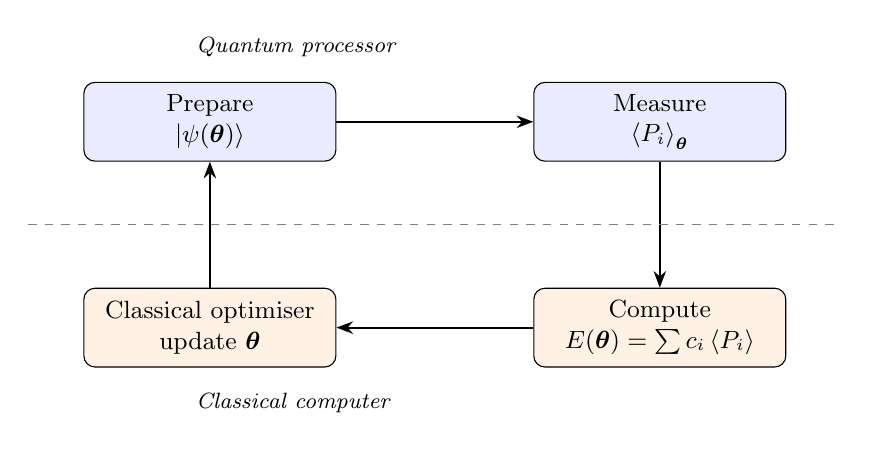
\begin{tikzpicture}[
    node distance=1.6cm and 2.5cm,
    box/.style={
      draw, rounded corners=4pt, minimum width=3.2cm,
      minimum height=1cm, align=center, font=\small
    },
    arrow/.style={-{Stealth[length=6pt]}, thick},
  ]
  \node[box, fill=blue!8] (prep) {Prepare\\$\ket{\psi(\bm{\theta})}$};
  \node[box, fill=blue!8, right=of prep] (meas)
    {Measure\\$\expval{P_i}_{\bm{\theta}}$};
  \node[box, fill=orange!10, below=of meas] (eval)
    {Compute\\$E(\bm{\theta})=\sum c_i\expval{P_i}$};
  \node[box, fill=orange!10, below=of prep] (opt)
    {Classical optimiser\\update $\bm{\theta}$};

  \draw[arrow] (prep) -- (meas);
  \draw[arrow] (meas) -- (eval);
  \draw[arrow] (eval) -- (opt);
  \draw[arrow] (opt) -- (prep);

  \node[font=\footnotesize\itshape, above=0.2cm of prep, anchor=south west,
        xshift=-0.3cm] {Quantum processor};
  \node[font=\footnotesize\itshape, below=0.2cm of opt, anchor=north west,
        xshift=-0.3cm] {Classical computer};

  \draw[dashed, gray] ($(prep.south west)+(-0.7,-0.8)$) --
                       ($(meas.south east)+(0.7,-0.8)$);
\end{tikzpicture}
\caption{The hybrid variational loop. The quantum processor prepares a
  parameterised state and estimates the Pauli expectation values that
  compose the energy; the classical optimiser proposes the next
  $\bm{\theta}$. The cost function is a statistical average over circuit
  shots, which is what makes the loop robust to the gate errors of NISQ
  hardware.}
\label{fig:vqe_loop}
\end{figure}

The remainder of this section explains \emph{why} this hybrid arrangement
is the right framework for present-day hardware, and where its limits
lie. Two properties are responsible for both its success and its
characteristic failure modes: the noise resilience of an averaged cost
function, and the tension between the expressibility of a parameterised
ansatz and its trainability.

\subsection{Why the variational principle survives noise}
\label{sec:vqa_noise}

The decisive feature of a variational algorithm is that the quantity it
optimises is a statistical average. A single circuit shot returns a
bit-string. The cost $E(\bm{\theta})$ is the empirical mean of many such
shots, weighted by the Pauli coefficients of $H$. Stochastic shot noise
and biased gate errors therefore enter the optimiser as a deformation of
the cost landscape, not as a corrupted coherent observable that must
survive intact to the final measurement.

Two consequences follow. First, depolarising-like noise of strength $p$
applied uniformly across the circuit damps every nontrivial Pauli
expectation by a common factor that depends on the circuit structure but
not on $\bm{\theta}$ once the optimiser sits near a smooth minimum. The
position of the minimum in parameter space is preserved, while the
absolute energy at that minimum is biased upward by an amount that can be
estimated and partially removed by zero-noise extrapolation. Second, the
optimiser is insensitive to constant offsets in the cost: any
$\bm{\theta}$-independent shift cancels under finite differences and
gradient updates. This is the formal sense in which variational
algorithms are self-correcting against coherent miscalibration, and it is
the property that justifies their use on devices whose two-qubit gate
infidelities sit orders of magnitude above the fault-tolerance
threshold~\cite{mcclean2016,preskill2018}.

The contrast with quantum phase estimation is informative. Phase
estimation reads the ground-state energy off the relative phase of an
ancilla, accumulated coherently over a sequence of controlled-$U$
applications whose length scales with the desired precision. A single
decohering event in that sequence corrupts the phase and the answer.
Variational methods replace this brittle coherent encoding by an
incoherent average, paying a $1/\sqrt{N_{\mathrm{shots}}}$ statistical
cost in exchange for graceful degradation under the noise budget of NISQ
hardware.

\subsection{Expressibility and trainability}
\label{sec:vqa_expressibility}

The flip side of this resilience is that the answer is only as good as
the ansatz. Two notions sharpen the question of how to choose
$U(\bm{\theta})$.

\emph{Expressibility} measures the extent to which the parameterised
manifold $\{U(\bm{\theta})\ket{0}^{\otimes n} : \bm{\theta}\in\mathbb{R}^p\}$
covers the physically relevant subspace of Hilbert space. If the true
ground state lies outside this manifold, the variational minimum is a
strict upper bound on $E_0$, and that bound cannot be tightened by more
optimiser iterations or more shots. Hardware-efficient ansatze chase
expressibility through depth: every additional layer of entangling gates
and single-qubit rotations enlarges the reachable manifold.

\emph{Trainability} measures the conditioning of the cost landscape.
A maximally expressive ansatz on $n$ qubits suffers the barren-plateau
phenomenon~\cite{mcclean2018,cerezo2021}: the variance of the energy
gradient with respect to any single parameter decays exponentially in $n$,
so the landscape is essentially flat across the bulk of parameter space
and the optimiser receives no signal. Pushing for more expressibility
through brute depth therefore destroys trainability, yielding ansatze
that can in principle reach the ground state but cannot be steered there.

The way out is to give up universal coverage in favour of
problem-specific symmetries. A particle-number-conserving manifold, for
instance, restricts the search to the physically meaningful sector and
shrinks the parameter space by orders of magnitude, restoring nonzero
gradients. The Unitary Coupled Cluster ansatz used by Gallimore and Liao
(\cref{sec:gallimore}) and the three-parameter $R_y$ ansatz used by
Woloshyn (\cref{sec:woloshyn}) are both instances of this strategy: each
is tailored to its qubit encoding so that the trial manifold contains
the ground state of the channel Hamiltonian while remaining
low-dimensional enough to be trainable on current hardware.

Beyond the ground state, the same hybrid framework extends naturally:
orthogonality penalties give access to excited states, imaginary-time
equations of motion give a noise-stable route to the ground state from
arbitrary starting points, and parameterised propagators give dynamical
observables. The three algorithms developed in the next chapter cover
precisely these three extensions on the same charmonium Hamiltonian,
making the strengths and limits of the variational framework visible in
a single physical system.


% ──────────────────────────────────────────────────────────────────
\section{Thesis Overview}
\label{sec:overview}

This thesis applies three variational quantum algorithms to charmonium
spectroscopy, comparing them on the same ${}^1S_0$, ${}^3S_1$, and
${}^1P_1$ channel Hamiltonians and on the same noise model. The goal is
to test whether the variational framework introduced in this chapter can
recover spin-dependent mass splittings of the charmonium spectrum on
hardware whose fidelity is firmly within the NISQ regime, and to
identify which features of each algorithm carry that performance.

The remaining chapters are organised as follows:
\begin{itemize}
  \item \textbf{Chapter~2} introduces the charmonium system, derives the
    radial Hamiltonian in a truncated harmonic-oscillator basis, and
    develops in self-contained form the three algorithms studied in this
    thesis: the Variational Quantum Eigensolver of Gallimore and Liao,
    the Variational Imaginary-Time Evolution method of Woloshyn, and the
    Trotter--Taylor Imaginary-Time Evolution scheme of Yi et al.
  \item \textbf{Chapter~3} presents the numerical results: noiseless
    benchmarks of energies and transition amplitudes, and the
    noisy-simulator study that quantifies how each algorithm degrades
    under depolarising gate noise.
\end{itemize}


% ══════════════════════════════════════════════════════════════════
\chapter{Mathematical Framework and Quantum Algorithms}
\label{ch:framework}

This chapter develops the mathematical machinery that the remainder of the
thesis relies on. We begin in \cref{sec:hamiltonian} by constructing the
charmonium Hamiltonian in a truncated harmonic-oscillator basis, treating the
three channels of interest---${}^1S_0$, ${}^3S_1$, and ${}^1P_1$---on equal
footing. \Cref{sec:encoding} then encodes the resulting matrix on a quantum
register through two complementary schemes: a compact direct mapping and a
Jordan--Wigner mapping of an underlying second-quantised representation. The
three quantum algorithms used throughout this work are introduced in turn:
the Variational Quantum Eigensolver (\cref{sec:vqe}), Variational
Imaginary-Time Evolution (\cref{sec:vqite}), and the probabilistic
Trotter--Taylor Imaginary-Time Evolution scheme (\cref{sec:ttite}). Beyond
energy spectra, observable physical predictions also require transition
amplitudes; \cref{sec:transitions} develops the quantum-circuit techniques for
estimating M1 and E1 transitions between channels. We close
(\cref{sec:framework-summary}) with a side-by-side comparison of the three
algorithms.

We follow the treatments of Gallimore and Liao~\cite{gallimore2023},
Woloshyn~\cite{woloshyn2023}, and Yi et al.~\cite{yi2025}, adapting each to a
common setting: the spin-dependent charmonium spectrum represented in a
four-state harmonic-oscillator basis.

% ──────────────────────────────────────────────────────────────────
\section{The Charmonium Hamiltonian}
\label{sec:hamiltonian}

We begin by writing the charmonium Hamiltonian in a form amenable to numerical
diagonalisation. The starting point is the non-relativistic quark model with
a Cornell potential and a leading spin-dependent correction; the strategy is
to expand the radial wavefunction in a finite harmonic-oscillator basis,
producing a finite matrix whose lowest eigenvalues approximate the physical
energy levels.

\subsection{The non-relativistic quark model}
\label{ssec:quark_model}

A charmonium meson is a bound state of a charm quark and its
antiquark~\cite{eichten1978,brambilla2011}. Because the charm mass
$m_c \simeq 1.48~\mathrm{GeV}/c^2$ is large compared with the binding energy,
the internal motion is well described non-relativistically: the relative
coordinate $\mathbf{r} = \mathbf{r}_c - \mathbf{r}_{\bar c}$ satisfies the
two-body Schr\"{o}dinger equation
\begin{equation}
  \label{eq:two_body}
  H\,\psi(\mathbf{r}) =
    \left[-\frac{\nabla^{2}}{2\mu} + V(r)\right]\psi(\mathbf{r})
    = E\,\psi(\mathbf{r}),
\end{equation}
with reduced mass $\mu = m_c/2$. The interaction $V(r)$ has two pieces.
The first is the spin-independent Cornell potential
\begin{equation}
  \label{eq:cornell_potential}
  V_0(r) = -\frac{a}{r} + b\,r,
  \qquad a = \frac{4\alpha_s}{3},
\end{equation}
where $-a/r$ is the colour-Coulomb attraction from one-gluon exchange and
$b\,r$ is the linearly rising flux-tube term that confines the
quarks~\cite{eichten1978}. The second piece is the leading spin-dependent
correction. From the non-relativistic reduction of the Breit interaction,
the dominant term at one-gluon-exchange order is the contact
(hyperfine) interaction~\cite{barnes2005,brambilla2011}
\begin{equation}
  \label{eq:hyperfine}
  V_s(r) =
    \frac{32\pi\,\alpha_s}{9\,m_c^{2}}\,
    \delta_\sigma(\mathbf{r})\,
    \mathbf{S}_c\cdot\mathbf{S}_{\bar c},
\end{equation}
where we have replaced the singular Dirac delta with a normalised Gaussian of
width $\sigma$,
\begin{equation}
  \label{eq:gaussian_delta}
  \delta_\sigma(\mathbf{r}) =
    \left(\frac{\sigma}{\sqrt{\pi}}\right)^{3} e^{-\sigma^{2} r^{2}},
\end{equation}
to regularise the contact term inside our finite basis. The dot product of
the two quark spin operators is fixed by the total spin
$\mathbf{S} = \mathbf{S}_c + \mathbf{S}_{\bar c}$ through the identity
$\mathbf{S}^{2} = \mathbf{S}_c^{2} + \mathbf{S}_{\bar c}^{2}
 + 2\,\mathbf{S}_c\cdot\mathbf{S}_{\bar c}$, giving
\begin{equation}
  \label{eq:spin_dot}
  \mathbf{S}_c\cdot\mathbf{S}_{\bar c} =
  \begin{cases}
    -\tfrac{3}{4} & \text{spin singlet } (S=0),\\[4pt]
    +\tfrac{1}{4} & \text{spin triplet } (S=1).
  \end{cases}
\end{equation}
The phenomenological parameters $\alpha_s$, $b$, $m_c$, and $\sigma$ used
throughout this work are those of Barnes, Godfrey, and
Swanson~\cite{barnes2005} and are listed in \cref{tab:cornell_params}.

\begin{table}[htbp]
\centering
\caption{Cornell-potential parameters used in this work, following the
  charmonium fit of Barnes, Godfrey, and Swanson~\cite{barnes2005}. The
  conversion $\hbar c = 197.326$~MeV$\cdot$fm relates inverse-femtometres to
  MeV. The Coulomb coefficient is $a = 4\alpha_s/3$.}
\label{tab:cornell_params}
\begin{tabular}{lll}
\toprule
Parameter & Symbol & Value \\
\midrule
Strong coupling          & $\alpha_s$    & $0.5461$ \\
String tension           & $b$           & $0.1425~\mathrm{GeV}^{2}$ \\
Charm-quark mass         & $m_c$         & $1.4794~\mathrm{GeV}$ \\
Gaussian width           & $\sigma$      & $1.0946~\mathrm{GeV}$ \\
\bottomrule
\end{tabular}
\end{table}

\subsection{Radial equation and the three channels}
\label{ssec:channels}

Because $V_0(r)$ depends only on $r = |\mathbf{r}|$ and the spin operator in
\cref{eq:hyperfine} commutes with the orbital angular momentum, eigenstates
of $H$ can be classified by the spectroscopic quantum numbers
${}^{2S+1}L_J$. Writing the wavefunction as
\begin{equation}
  \label{eq:separation}
  \psi(\mathbf{r}) = R_{n\ell}(r)\,Y_{\ell m}(\hat{\mathbf{r}})\,\chi_{S M_S},
\end{equation}
and defining the reduced radial function $u_{n\ell}(r) = r R_{n\ell}(r)$, the
Schr\"{o}dinger equation reduces to the one-dimensional eigenvalue problem
\begin{equation}
  \label{eq:radial}
  \left[
    -\frac{1}{2\mu}\frac{\mathrm{d}^{2}}{\mathrm{d}r^{2}}
    + V_0(r)
    + \frac{\ell(\ell+1)}{2\mu r^{2}}
    + \langle\mathbf{S}_c\cdot\mathbf{S}_{\bar c}\rangle\,
      \frac{32\pi\alpha_s}{9 m_c^{2}}\,\delta_\sigma(r)
  \right] u_{n\ell}(r) = E_{n\ell}\,u_{n\ell}(r),
\end{equation}
where the centrifugal barrier $\ell(\ell+1)/(2\mu r^2)$ is the standard
remnant of the angular Laplacian, and the spin expectation value takes the
discrete values of \cref{eq:spin_dot}.

In this work we focus on the three low-lying channels that have served as
benchmarks for quantum simulations of quarkonium~\cite{woloshyn2023}:
\begin{itemize}
  \item ${}^1S_0$ (associated with the $\eta_c$ meson): $\ell=0$, $S=0$. The
    centrifugal barrier vanishes and the contact term contributes with
    $\langle\mathbf{S}_c\cdot\mathbf{S}_{\bar c}\rangle = -3/4$.
  \item ${}^3S_1$ (associated with the $J/\psi$ meson): $\ell=0$, $S=1$. As
    for ${}^1S_0$ but with $\langle\mathbf{S}_c\cdot\mathbf{S}_{\bar c}\rangle
    = +1/4$, producing the celebrated $\eta_c$--$J/\psi$ hyperfine splitting.
  \item ${}^1P_1$ (associated with the $h_c$ meson): $\ell=1$, $S=0$. The
    contact term contributes only at the origin, and because the
    $\ell=1$ wavefunction vanishes there the spin-dependent term is
    numerically negligible for $P$-waves; the centrifugal barrier, however,
    shifts the energies up substantially.
\end{itemize}
Each channel thus generates a different one-dimensional radial Hamiltonian,
which we now discretise.

\subsection{Harmonic-oscillator basis expansion}
\label{ssec:ho_basis}

The radial functions $u_{n\ell}(r)$ admit a convenient expansion in the
eigenstates of a three-dimensional isotropic harmonic oscillator (HO),
\begin{equation}
  \label{eq:ho_states}
  \phi_{n\ell}(r) =
    N_{n\ell}\,r^{\ell+1}\,
    \exp\!\left(-\frac{r^{2}}{2 b^{2}}\right)
    L_{n}^{\ell + 1/2}\!\left(\frac{r^{2}}{b^{2}}\right),
\end{equation}
with normalisation
\(N_{n\ell} = \sqrt{2\,n!\, b^{-(2\ell+3)} /\,\Gamma(n+\ell+3/2)}\)
and $L_n^{\alpha}$ the associated Laguerre polynomials. The length scale
$b = (\mu\omega)^{-1/2}$ is determined by the oscillator frequency $\omega$,
which is chosen variationally so that the ground state of the basis already
captures most of the physical ground-state wavefunction~\cite{gallimore2023}.

We truncate the basis to the first $N=4$ states for each channel,
\begin{equation}
  \label{eq:basis_expansion}
  u_{n\ell}(r) \;\approx\; \sum_{k=0}^{N-1} c_k^{(n)}\,\phi_{k\ell}(r),
  \qquad N = 4,
\end{equation}
which turns \cref{eq:radial} into the finite-dimensional eigenvalue problem
\begin{equation}
  \label{eq:matrix_problem}
  \sum_{k=0}^{N-1} H_{mk}^{(\ell,S)}\,c_k^{(n)} = E_n\,c_m^{(n)},
\end{equation}
where the channel-dependent matrix elements are
\begin{equation}
  \label{eq:matrix_elements}
  H_{mk}^{(\ell,S)} =
    \langle\phi_{m\ell}|\,T\,|\phi_{k\ell}\rangle
    + \langle\phi_{m\ell}|\,V_0\,|\phi_{k\ell}\rangle
    + \langle\mathbf{S}_c\cdot\mathbf{S}_{\bar c}\rangle\,
      \frac{32\pi\alpha_s}{9 m_c^{2}}\,
      \langle\phi_{m\ell}|\,\delta_\sigma\,|\phi_{k\ell}\rangle.
\end{equation}
Here $T$ denotes the kinetic term plus, for $\ell>0$, the centrifugal barrier.

\begin{remark}[Hylleraas--Undheim--MacDonald theorem]
The truncation in \cref{eq:basis_expansion} introduces a controlled
approximation: the eigenvalues of the truncated matrix
$H^{(\ell,S)} \in \mathbb{R}^{N\times N}$ are guaranteed to be upper
bounds on the corresponding exact eigenvalues, and they are monotonically
non-increasing in $N$~\cite{macdonald1933}. Increasing $N$ therefore
always improves the variational estimate; $N=4$ provides a useful balance
between physical accuracy and the qubit cost of the encodings introduced
in \cref{sec:encoding}.
\end{remark}

\subsection{Matrix elements}
\label{ssec:matrix_elements}

The matrix elements in \cref{eq:matrix_elements} can be evaluated in closed
form using standard identities for the Laguerre polynomials and the
hypergeometric function. We collect the key results here; complete derivations
follow the methodology of Gallimore and Liao~\cite{gallimore2023}.

\paragraph{Kinetic energy.}
The kinetic operator, expressed through the ladder operators of the
oscillator, is tridiagonal in the HO basis. For $\ell=0$ one finds
\begin{equation}
  \label{eq:kinetic_matrix}
  \langle m | T | k \rangle = \frac{\omega}{2}\Bigl[
    \bigl(2k + \tfrac{3}{2}\bigr)\delta_{mk}
    -\sqrt{k(k+\tfrac{1}{2})}\,\delta_{m,k-1}
    -\sqrt{(k+1)(k+\tfrac{3}{2})}\,\delta_{m,k+1}
  \Bigr].
\end{equation}
For $\ell>0$ the centrifugal term is absorbed into a shifted diagonal,
$2k + \ell + 3/2$, with the off-diagonal couplings inheriting the same
square-root structure with the index $\ell + 1/2$ in place of $1/2$.

\paragraph{Coulomb term.}
The matrix element of $1/r$ can be expressed in terms of a generalised
hypergeometric function ${}_3F_2$~\cite{gallimore2023}:
\begin{equation}
  \label{eq:coulomb_matrix}
  \langle m | r^{-1} | k \rangle =
    \frac{(-1)^{m+k}\,4 b^{-1}}{\pi (1 + 2k)}
    \sqrt{\frac{\Gamma(m+\tfrac{3}{2})\,\Gamma(k+\tfrac{3}{2})}{m!\,k!}}\,
    {}_3F_2\!\left(\tfrac{1}{2},1,-m;\;\tfrac{3}{2},\tfrac{1}{2}-k;\;1\right).
\end{equation}

\paragraph{Linear-confinement term.}
The matrix element of $r$ involves the Gauss hypergeometric ${}_2F_1$:
\begin{equation}
  \label{eq:linear_matrix}
  \langle m | r | k \rangle =
    \frac{(-1)^{m+k}\,4 b}{\pi (1 - 4k^{2})}
    \sqrt{\frac{\Gamma(m+\tfrac{3}{2})\,\Gamma(k+\tfrac{3}{2})}{m!\,k!}}\,
    {}_2F_1\!\left(2,-m;\;\tfrac{3}{2}-k;\;1\right).
\end{equation}

\paragraph{Contact term.}
For the regularised contact interaction with the Gaussian of
\cref{eq:gaussian_delta}, the matrix element reduces to a single Gaussian
integral over a polynomial in $r^{2}$, which is again closed-form:
\begin{equation}
  \label{eq:contact_matrix}
  \langle\phi_{m\ell}|\,\delta_\sigma\,|\phi_{k\ell}\rangle
  = \left(\frac{\sigma}{\sqrt{\pi}}\right)^{3}\!\!
    \int_0^{\infty}\!\!\phi_{m\ell}(r)\,e^{-\sigma^{2} r^{2}}\,
    \phi_{k\ell}(r)\,\mathrm{d}r.
\end{equation}
For $\ell>0$ the factor $r^{2\ell+2}$ in the integrand suppresses the
contribution near the origin; in the limit $\sigma\to\infty$ the integral
vanishes for $\ell>0$ and reproduces $|\phi_{m\ell}(0)\phi_{k\ell}(0)|$
for $\ell=0$, recovering the unregularised Dirac-delta result.

\begin{remark}
The signs $(-1)^{m+k}$ in \cref{eq:coulomb_matrix,eq:linear_matrix} encode
the alternating parity of the Laguerre polynomials at the origin and are
essential for obtaining the correct off-diagonal Cornell-potential matrix
elements. In practice all of these closed-form expressions are evaluated to
high precision via the \texttt{mpmath} library and verified against direct
numerical quadrature.
\end{remark}

\subsection{The three Hamiltonian matrices}
\label{ssec:matrices}

Assembling \cref{eq:matrix_elements} channel by channel with the parameters
of \cref{tab:cornell_params} and $\omega = 1.2~\mathrm{fm}^{-1}$ produces the
following three $4\times 4$ matrices (in units of $\mathrm{fm}^{-1}$, with
conversion to MeV via $\hbar c = 197.326~\mathrm{MeV}\!\cdot\!\mathrm{fm}$):
\begin{align}
H^{({}^1S_0)} &= \begin{pmatrix}
   0.9431 & -0.8733 & -0.7690 & -0.5601\\
  -0.8733 &  3.3365 & -0.5646 & -0.8648\\
  -0.7690 & -0.5646 &  5.4382 & -0.1566\\
  -0.5601 & -0.8648 & -0.1566 &  7.3451
\end{pmatrix},
\label{eq:H_1S0}\\[4pt]
H^{({}^3S_1)} &= \begin{pmatrix}
   1.0946 & -0.7114 & -0.6111 & -0.4112\\
  -0.7114 &  3.5406 & -0.3910 & -0.6989\\
  -0.6111 & -0.3910 &  5.6122 & -0.0119\\
  -0.4112 & -0.6989 & -0.0119 &  7.5104
\end{pmatrix},
\label{eq:H_3S1}\\[4pt]
H^{({}^1P_1)} &= \begin{pmatrix}
   2.8561 & -0.2395 & -0.3827 & -0.2282\\
  -0.2395 &  4.9190 & -0.0373 & -0.5097\\
  -0.3827 & -0.0373 &  6.8114 &  0.4058\\
  -0.2282 & -0.5097 &  0.4058 &  8.6034
\end{pmatrix}.
\label{eq:H_1P1}
\end{align}
Each matrix is real and symmetric, a consequence of the Hermiticity of the
underlying operator and the choice of real-valued HO basis functions. The
${}^1P_1$ matrix lies higher in absolute energy because of the
$\ell=1$ centrifugal contribution to the diagonal; the spin-dependent shift
between ${}^1S_0$ and ${}^3S_1$ is visible already in the difference between
their diagonal entries.

\begin{remark}[Errata in the literature]
We note that in the published matrices for ${}^1P_1$~\cite{woloshyn2023} the
$(3,3)$ element was reported as $7.5104$, coinciding numerically with the
$(3,3)$ entry of $H^{({}^3S_1)}$. Cross-checking against the variational
eigenvalues and the diagonal pattern of the kinetic + centrifugal +
confinement contributions identifies this as a copy-paste error; the correct
value $8.6034$ is used in \cref{eq:H_1P1}.
\end{remark}

Diagonalising each $H^{(\ell,S)}$ by classical means immediately yields the
exact (within the truncated basis) energy spectrum of its channel. Doing so on
a quantum computer, however, requires representing the operator as a sum of
Pauli strings acting on a register of qubits, which is the topic of the next
section.


% ──────────────────────────────────────────────────────────────────
\section{Encoding the Hamiltonian on Qubits}
\label{sec:encoding}

To run a quantum algorithm we must express the channel Hamiltonians
\cref{eq:H_1S0,eq:H_3S1,eq:H_1P1} in a form that the device can act on
natively: a sum of tensor products of Pauli operators acting on a finite
register of qubits. Two qualitatively different encoding choices appear in
the literature for this kind of basis-expansion problem, and we will use
both later in the thesis. This section derives them in parallel for the
same underlying $4\times 4$ matrices, allowing a direct comparison of qubit
count and Pauli structure.

\subsection{Pauli decomposition of a Hermitian matrix}
\label{ssec:pauli_decomp}

Any Hermitian operator $H$ on $n$ qubits can be written as a real linear
combination of the $4^{n}$ Pauli strings
$\{P_k\} \subset \{I,X,Y,Z\}^{\otimes n}$,
\begin{equation}
  \label{eq:pauli_sum}
  H = \sum_{k=1}^{4^{n}} c_k\,P_k,
  \qquad c_k = \frac{1}{2^{n}}\,\Tr(H\,P_k)\in\mathbb{R}.
\end{equation}
The relation \cref{eq:pauli_sum} follows from the orthogonality of Pauli
strings under the Hilbert--Schmidt inner product,
$\Tr(P_j P_k) = 2^{n}\delta_{jk}$. In practice only a small subset of the
$4^{n}$ coefficients are nonzero; for real symmetric Hamiltonians, all
strings containing an odd number of $Y$ factors vanish identically, leaving
$3^{n}$ candidate terms.

Once $H$ has been put in the form \cref{eq:pauli_sum}, each Pauli string can
be implemented as a basis rotation on the quantum register followed by a
diagonal measurement, and the expectation value $\langle H\rangle$ recovered
as the weighted sum $\sum_k c_k\langle P_k\rangle$. The remaining question
is which qubit register to use---i.e., how to associate physical basis
states with bit-strings. We discuss two natural choices.

\subsection{Direct (compact) encoding}
\label{ssec:direct_encoding}

The most economical scheme assigns one bit-string to each HO basis
function via the binary expansion of its index,
\begin{equation}
  \label{eq:direct_map}
  |n\rangle_{\mathrm{HO}}
  \;\longmapsto\;
  |\mathrm{bin}(n)\rangle_{\mathrm{qubit}},
  \qquad n = 0,1,2,3.
\end{equation}
For $N=4$ this requires only $\lceil\log_2 N\rceil = 2$ qubits, and every
computational-basis state of the register corresponds to a physical HO state.
In particular,
\begin{equation}
  |0\rangle \mapsto |00\rangle,\quad
  |1\rangle \mapsto |01\rangle,\quad
  |2\rangle \mapsto |10\rangle,\quad
  |3\rangle \mapsto |11\rangle.
\end{equation}
The channel Hamiltonian $H^{(\ell,S)}$ is then literally a $4\times 4$ matrix
acting on this register, and its Pauli decomposition follows from
\cref{eq:pauli_sum}. Applying that formula to the ${}^1S_0$ matrix of
\cref{eq:H_1S0} yields, for example,
\begin{equation}
  \label{eq:direct_decomp_1S0}
  H^{({}^1S_0)} =
  c_{II}\,II + c_{IZ}\,IZ + c_{ZI}\,ZI + c_{ZZ}\,ZZ
  + c_{IX}\,IX + c_{XI}\,XI + c_{ZX}\,ZX + c_{XZ}\,XZ
  + c_{XX}\,XX + c_{YY}\,YY,
\end{equation}
i.e.\ ten Pauli terms, consistent with the absence of strings containing a
single $Y$ for a real-symmetric operator. The numerical coefficients
$\{c_k\}$ are obtained by trace formulas and are real.

\begin{example}[Identity coefficient]
Setting $P_k = I\otimes I$ in \cref{eq:pauli_sum} gives the energy offset
\[
  c_{II} = \frac{1}{4}\Tr H^{({}^1S_0)}
         = \frac{1}{4}(0.9431 + 3.3365 + 5.4382 + 7.3451) \approx 4.266,
\]
which simply records the trace of the channel matrix and contributes only a
constant shift to the eigenvalues.
\end{example}

The direct encoding has two clear advantages: it uses the minimal number of
qubits, and every computational-basis state is physical, so the variational
ansatz need not respect any external constraint. Its main drawback is that
the resulting Pauli strings carry no obvious physical interpretation---they
are simply the coefficients of an abstract $4\times 4$ matrix.

\subsection{Jordan--Wigner (occupation) encoding}
\label{ssec:jw_encoding}

The second encoding originates in quantum chemistry. We treat the HO basis
functions as orbitals occupied by a single charm--anticharm pair and
introduce a fermionic creation operator $a_n^{\dagger}$ for each orbital, with
the canonical anticommutation relations
\begin{equation}
  \label{eq:fermion_anticom}
  \{a_m, a_n^{\dagger}\} = \delta_{mn},
  \qquad
  \{a_m, a_n\} = \{a_m^{\dagger}, a_n^{\dagger}\} = 0.
\end{equation}
The channel Hamiltonian is then the second-quantised one-body operator
\begin{equation}
  \label{eq:second_quantised}
  \widehat{H}^{(\ell,S)} =
    \sum_{m,n=0}^{N-1} H_{mn}^{(\ell,S)}\;a_m^{\dagger} a_n,
\end{equation}
acting on the Fock space of $N=4$ orbitals; physical states are those
containing exactly one excitation, i.e.\ the four states
$\{a_n^{\dagger}|\mathrm{vac}\rangle\}_{n=0}^{3}$. Restricting to this
single-particle sector reproduces the original $4\times 4$ matrix problem.

\paragraph{Jordan--Wigner transformation.}
The Jordan--Wigner (JW) transformation~\cite{nielsen2010} maps each orbital
to a dedicated qubit and faithfully reproduces the fermionic algebra
\cref{eq:fermion_anticom} in terms of Pauli operators,
\begin{align}
  \label{eq:jw_a_dagger}
  a_n^{\dagger} &=
    \frac{1}{2}\,\Bigl(\,\prod_{j<n} Z_j\Bigr)\,(X_n - i\,Y_n),\\[3pt]
  \label{eq:jw_a}
  a_n &=
    \frac{1}{2}\,\Bigl(\,\prod_{j<n} Z_j\Bigr)\,(X_n + i\,Y_n).
\end{align}
The trailing string of $Z$ operators on lower-indexed qubits encodes the
fermionic sign that arises when a creation operator anticommutes past
already-occupied orbitals. With this mapping, $N=4$ orbitals require $N=4$
qubits, of which only $\binom{4}{1}=4$ computational-basis states are
physical (namely $|0001\rangle,|0010\rangle,|0100\rangle,|1000\rangle$).

\paragraph{Pauli forms of the one-body operators.}
Substituting \cref{eq:jw_a_dagger,eq:jw_a} into the bilinears
$a_m^{\dagger} a_n$ yields concrete Pauli strings. The number operator at
orbital $n$ is diagonal,
\begin{equation}
  \label{eq:jw_number}
  a_n^{\dagger} a_n = \frac{1}{2}(I - Z_n).
\end{equation}
Adjacent hopping ($|m-n|=1$, e.g.\ between orbitals $n$ and $n+1$) gives the
familiar $XX{+}YY$ pattern,
\begin{equation}
  \label{eq:jw_adjacent}
  a_n^{\dagger} a_{n+1} + a_{n+1}^{\dagger} a_n
  = \frac{1}{2}\bigl(X_n X_{n+1} + Y_n Y_{n+1}\bigr),
\end{equation}
while non-adjacent hops pick up the JW $Z$-string,
\begin{align}
  \label{eq:jw_skip1}
  a_n^{\dagger} a_{n+2} + a_{n+2}^{\dagger} a_n
    &= \frac{1}{2}\bigl(X_n Z_{n+1} X_{n+2} + Y_n Z_{n+1} Y_{n+2}\bigr),\\
  \label{eq:jw_skip2}
  a_n^{\dagger} a_{n+3} + a_{n+3}^{\dagger} a_n
    &= \frac{1}{2}\bigl(X_n Z_{n+1} Z_{n+2} X_{n+3}
                       + Y_n Z_{n+1} Z_{n+2} Y_{n+3}\bigr).
\end{align}
Combining these expressions with the coefficients $H_{mn}^{(\ell,S)}$ from
\cref{eq:H_1S0,eq:H_3S1,eq:H_1P1} produces a Pauli-string decomposition of
$\widehat{H}^{(\ell,S)}$.

\paragraph{Term counting.}
Collecting all distinct strings for $N=4$, the Jordan--Wigner Hamiltonian
contains
\begin{itemize}\setlength{\itemsep}{2pt}
  \item one identity term (energy offset, from the diagonals through
    $a_n^{\dagger} a_n$);
  \item four single-qubit $Z$ terms (one per orbital, from the diagonals);
  \item six pairs of $XX{+}YY$, $XZX{+}YZY$, or $XZZX{+}YZZY$ strings (one
    pair per off-diagonal element of $H^{(\ell,S)}$).
\end{itemize}
The total is $1 + 4 + 12 = 17$ Pauli strings, compared with the ten of the
direct encoding. The two extra orbitals---and the corresponding $Z$-string
overhead in \cref{eq:jw_skip2}---are the price paid for the physically
transparent occupation-number picture.

\begin{remark}[Reduction to Gallimore's $N=3$ case]
Gallimore and Liao~\cite{gallimore2023} applied the JW construction to a
\emph{spin-independent} Cornell potential truncated to $N=3$ basis states,
producing a $3\times 3$ Hamiltonian on $3$ qubits with $10$ Pauli terms.
The construction above extends that procedure in two directions: we
include the spin-dependent contact term of \cref{eq:hyperfine} and we use
$N=4$ basis functions. Restricting to $N=3$ and $\langle V_s\rangle = 0$
reproduces their decomposition exactly.
\end{remark}

\subsection{Comparison of the two encodings}
\label{ssec:encoding_compare}

\begin{table}[htbp]
\centering
\caption{Comparison of the two encodings of the channel Hamiltonians of
  \cref{eq:H_1S0,eq:H_3S1,eq:H_1P1} on a quantum register of qubits.}
\label{tab:encoding_compare}
\begin{tabular}{lcc}
\toprule
                 & Direct encoding              & Jordan--Wigner encoding \\
\midrule
Qubits           & $\lceil\log_2 N\rceil = 2$   & $N = 4$ \\
Physical states  & all $2^{2}=4$                 & only $\binom{4}{1}=4$ out of $16$ \\
Pauli terms      & $\sim 10$                     & $\sim 17$ \\
Ansatz constraint& none                          & single-particle sector \\
Physical picture & abstract                      & occupation of orbitals \\
\bottomrule
\end{tabular}
\end{table}

\Cref{tab:encoding_compare} summarises the trade-offs. The direct encoding
is more compact in qubit count and avoids any subspace constraint on the
variational ansatz, whereas the JW encoding offers a transparent connection
to second-quantised many-body methods and a natural framework for symmetry
preservation. Both encodings represent exactly the same physical Hamiltonian
in a different basis; the eigenvalues of \cref{eq:H_1S0,eq:H_3S1,eq:H_1P1}
are therefore identical in either picture. In what follows we adopt the
direct encoding as the default for compactness, switching to the JW
encoding when explicitly comparing it with Gallimore and
Liao~\cite{gallimore2023}.


% ──────────────────────────────────────────────────────────────────
\section{The Variational Quantum Eigensolver}
\label{sec:vqe}

With the Hamiltonian encoded as a Pauli sum, we now describe the simplest of
the three algorithms used in this thesis: the Variational Quantum Eigensolver
(VQE)~\cite{peruzzo2014,mcclean2016}. VQE is a direct application of the
Rayleigh--Ritz principle in which the trial state is prepared by a
parameterised quantum circuit and the energy is minimised by a classical
optimiser. The role of the quantum computer is to evaluate the expectation
value of an exponentially large Hamiltonian, a task that is in general
intractable classically; the optimisation itself is performed in the much
smaller classical parameter space.

\subsection{The variational principle, in operator form}
\label{ssec:vqe_principle}

For any Hermitian Hamiltonian $H$ on a finite Hilbert space, every
normalised state $\ket{\psi}$ obeys
\begin{equation}
  \label{eq:rayleigh_ritz}
  E_0 \;\leq\; \bra{\psi}H\ket{\psi},
\end{equation}
where $E_0$ is the smallest eigenvalue of $H$, with equality if and only if
$\ket{\psi}$ lies in the corresponding eigenspace. Restricting the search to
a family of \emph{trial states} $\{\ket{\psi(\bm{\theta})}\}$ parameterised by a
classical vector $\bm{\theta}\in\mathbb{R}^{p}$ gives the upper bound
\begin{equation}
  \label{eq:vqe_cost}
  E_0 \;\leq\;
  \min_{\bm{\theta}} \;
  E(\bm{\theta}),
  \qquad
  E(\bm{\theta}) \equiv \bra{\psi(\bm{\theta})} H \ket{\psi(\bm{\theta})}.
\end{equation}
The VQE algorithm computes $E(\bm{\theta})$ on the quantum processor and
minimises it on a classical computer; the resulting parameters
$\bm{\theta}^{\star}$ characterise an approximation $\ket{\psi(\bm{\theta}^{\star})}$
to the ground state.

The accuracy of this approximation is controlled by the
\emph{expressibility} of the ansatz: if the parameterised manifold
$\{\ket{\psi(\bm{\theta})}\}$ contains the true ground state then the minimum of
\cref{eq:vqe_cost} coincides with $E_0$; otherwise it provides a (variational)
upper bound. Two ansatz constructions are particularly natural for the
encodings of \cref{sec:encoding}.

\subsection{Ansatz for the direct encoding}
\label{ssec:woloshyn_ansatz}

For the two-qubit direct encoding of \cref{ssec:direct_encoding}, a state of
the form
\begin{equation}
  \label{eq:real_4state}
  \ket{\psi} = c_0\ket{00} + c_1\ket{01} + c_2\ket{10} + c_3\ket{11},
  \qquad c_n\in\mathbb{R},\;\sum_n c_n^{2} = 1,
\end{equation}
has three independent real degrees of freedom (four amplitudes minus the
normalisation). Because the channel Hamiltonians of
\cref{eq:H_1S0,eq:H_3S1,eq:H_1P1} are real and symmetric, their eigenstates
can be chosen real, and a three-parameter circuit producing the most general
real state of the form \cref{eq:real_4state} is therefore
expressible enough. Such a circuit, due to
Woloshyn~\cite{woloshyn2023}, applies two single-qubit $R_y$ rotations, a
CNOT, and a third $R_y$:
\begin{equation}
  \label{eq:direct_ansatz_op}
  U(\bm{\theta}) =
  \bigl[I \otimes R_y(\theta_2)\bigr]\,\mathrm{CNOT}_{0\to1}\,
  \bigl[R_y(\theta_1) \otimes R_y(\theta_0)\bigr],
\end{equation}
with $\bm{\theta} = (\theta_0,\theta_1,\theta_2)$. The corresponding circuit
is shown in \cref{fig:woloshyn_ansatz}.

\begin{figure}[htbp]
\centering
\begin{quantikz}
  \lstick{$\ket{0}$} & \gate{R_y(\theta_0)} & \ctrl{1} & \qw                 & \qw \\
  \lstick{$\ket{0}$} & \gate{R_y(\theta_1)} & \targ{}  & \gate{R_y(\theta_2)} & \qw
\end{quantikz}
\caption{Three-parameter ansatz used with the direct encoding. The two
  initial $R_y$ rotations create an arbitrary product state, the CNOT
  entangles the qubits, and the final $R_y$ provides the third independent
  degree of freedom required to reach a general real four-amplitude state.}
\label{fig:woloshyn_ansatz}
\end{figure}

Acting on $\ket{00}$, this circuit yields amplitudes
\begin{equation}
  \label{eq:direct_ansatz_state}
  \ket{\psi(\bm{\theta})} =
  \begin{pmatrix}
    c_0(c_1 c_2 - s_1 s_2)\\
    s_0(s_1 c_2 - c_1 s_2)\\
    c_0(c_1 s_2 + s_1 c_2)\\
    s_0(s_1 s_2 + c_1 c_2)
  \end{pmatrix},
  \qquad
  c_n = \cos(\theta_n/2),\; s_n = \sin(\theta_n/2),
\end{equation}
which can be verified to cover the unit sphere in $\mathbb{R}^{4}$ as
$\bm{\theta}$ ranges over a domain of size $4\pi^{3}$, modulo redundancies.

\subsection{Ansatz for the Jordan--Wigner encoding}
\label{ssec:ucc_ansatz}

For the four-qubit Jordan--Wigner encoding of \cref{ssec:jw_encoding} the
trial state must remain within the single-particle sector. A natural
construction starts from the reference state $\ket{0001}$ (one excitation in
the lowest orbital) and applies a unitary built from particle-conserving
operators. Extending the Unitary Coupled Cluster (UCC) ansatz of Gallimore
and Liao~\cite{gallimore2023} from $N=3$ to $N=4$ basis states, we define
\begin{equation}
  \label{eq:ucc_operator}
  U_{\mathrm{UCC}}(\theta_1,\theta_2,\theta_3) =
  \exp\!\left\{
    \sum_{k=1}^{3}\theta_k\,(a_k^{\dagger}a_0 - a_0^{\dagger}a_k)
  \right\}.
\end{equation}
Each generator $a_k^{\dagger}a_0 - a_0^{\dagger}a_k$ is anti-Hermitian and
preserves particle number, so $U_{\mathrm{UCC}}$ is unitary and maps
single-particle states to single-particle states. With three independent
parameters the operator generates the most general real superposition in the
single-particle sector,
\begin{equation}
  \label{eq:ucc_state}
  \ket{\psi(\alpha,\beta,\gamma)} =
    \cos\alpha\,\ket{0001}
    + \sin\alpha\cos\beta\,\ket{0010}
    + \sin\alpha\sin\beta\cos\gamma\,\ket{0100}
    + \sin\alpha\sin\beta\sin\gamma\,\ket{1000},
\end{equation}
which is simply the $\mathbb{S}^{3}$ spherical parameterisation lifted into
the single-particle sector. The trigonometric reparameterisation
$(\theta_1,\theta_2,\theta_3) \mapsto (\alpha,\beta,\gamma)$ is closed-form
but rarely needed in practice; the circuit is built directly from
\cref{eq:ucc_operator} using a sequence of Givens rotations between
adjacent orbitals~\cite{gallimore2023}. Compared with the direct-encoding
ansatz of \cref{fig:woloshyn_ansatz}, the UCC ansatz uses four qubits and a
deeper circuit, but it has the conceptual advantage of representing physical
particle hopping between HO orbitals.

\subsection{Measuring the energy on a quantum processor}
\label{ssec:vqe_measurement}

Given an ansatz $\ket{\psi(\bm{\theta})}$ and the Pauli decomposition
$H = \sum_k c_k P_k$ from \cref{eq:pauli_sum}, the energy estimator is
linear in the Pauli expectation values,
\begin{equation}
  \label{eq:vqe_energy_estimator}
  \widehat{E}(\bm{\theta}) = \sum_k c_k\,\langle P_k\rangle_{\bm{\theta}},
\end{equation}
where each $\langle P_k\rangle_{\bm{\theta}}$ is estimated separately by
preparing $\ket{\psi(\bm{\theta})}$ many times and measuring $P_k$.

A measurement in the computational basis directly gives access to
$\langle Z_i\rangle$, but $X$ and $Y$ observables require a basis rotation
applied before the measurement. The rotations are obtained from the
eigenbasis identities $X = H Z H$ and $Y = (S H) Z (H S^{\dagger})$, giving
the standard recipe
\begin{align}
  \label{eq:basis_rotations}
  \langle X_i\rangle &=
    \text{measure }Z_i \text{ after applying } H \text{ on qubit } i,\\[2pt]
  \langle Y_i\rangle &=
    \text{measure }Z_i \text{ after applying } S^{\dagger} H \text{ on qubit } i.
\end{align}
Each Pauli string $P_k$ is mapped to a diagonal observable by applying
these single-qubit basis rotations to every non-identity factor before the
final measurement.

\begin{remark}[Shot noise]
With a finite number $N_{\mathrm{shots}}$ of repetitions per circuit, the
estimator \cref{eq:vqe_energy_estimator} fluctuates around its true value with a
statistical uncertainty
\(
  \sigma_{\widehat{E}}
  = \sqrt{\sum_k c_k^{2}\,\sigma_{P_k}^{2} / N_{\mathrm{shots}}},
\)
where $\sigma_{P_k}^{2} \leq 1$ for any Pauli. The relative error therefore
decreases only as $1/\sqrt{N_{\mathrm{shots}}}$, which makes shot count an
important resource and motivates the choice of optimiser discussed next.
\end{remark}

\subsection{Classical optimisation}
\label{ssec:vqe_optimisation}

The cost function $\widehat{E}(\bm{\theta})$ is, in general, non-convex and
contaminated by shot noise. Two broad families of classical optimisers are
available:

\begin{itemize}\setlength{\itemsep}{2pt}
  \item \textbf{Gradient-free methods} (e.g.\ COBYLA, Nelder--Mead) only
    require evaluations of $\widehat{E}$ and are robust to moderate
    statistical noise. They typically converge in tens to a few hundreds of
    iterations for low-dimensional parameter spaces.
  \item \textbf{Gradient-based methods}, which require partial derivatives of
    $\widehat{E}$ at the cost of additional circuit evaluations. The
    \emph{parameter-shift rule} (\cref{sec:vqite}) provides exact analytic
    gradients for rotation gates, but each gradient component doubles the
    number of circuits.
\end{itemize}

For the few-parameter ansatze of
\cref{ssec:woloshyn_ansatz,ssec:ucc_ansatz} we use COBYLA throughout, which
balances simplicity, noise tolerance, and convergence speed.
\Cref{fig:vqe_loop_recap} recalls the resulting hybrid loop already
introduced in \cref{ch:introduction}: the classical optimiser proposes a
parameter update, the quantum processor evaluates
$\widehat{E}(\bm{\theta})$, and the cycle repeats until convergence.

\begin{figure}[htbp]
\centering
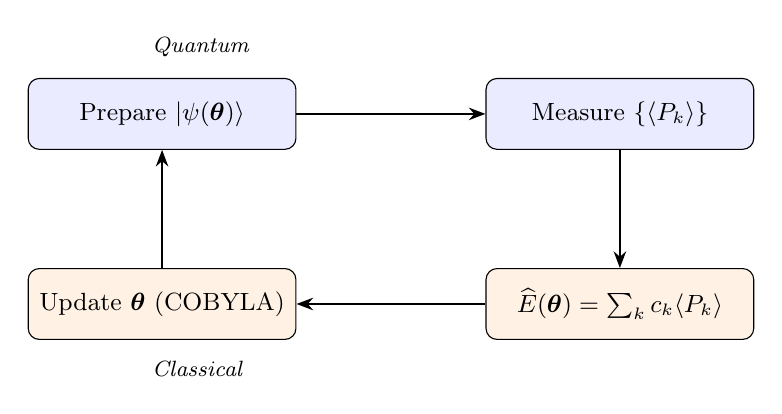
\begin{tikzpicture}[
    node distance=1.5cm and 2.4cm,
    box/.style={
      draw, rounded corners=4pt, minimum width=3.4cm,
      minimum height=0.9cm, align=center, font=\small
    },
    arrow/.style={-{Stealth[length=6pt]}, thick},
  ]
  \node[box, fill=blue!8] (prep) {Prepare $\ket{\psi(\bm{\theta})}$};
  \node[box, fill=blue!8, right=of prep] (meas)
    {Measure $\{\langle P_k\rangle\}$};
  \node[box, fill=orange!10, below=of meas] (eval)
    {$\widehat{E}(\bm{\theta}) = \sum_k c_k\langle P_k\rangle$};
  \node[box, fill=orange!10, below=of prep] (opt)
    {Update $\bm{\theta}$ (COBYLA)};
  \draw[arrow] (prep) -- (meas);
  \draw[arrow] (meas) -- (eval);
  \draw[arrow] (eval) -- (opt);
  \draw[arrow] (opt) -- (prep);
  \node[font=\footnotesize\itshape, above=0.15cm of prep, anchor=south west,
        xshift=-0.25cm] {Quantum};
  \node[font=\footnotesize\itshape, below=0.15cm of opt, anchor=north west,
        xshift=-0.25cm] {Classical};
\end{tikzpicture}
\caption{The VQE hybrid loop specialised to charmonium spectroscopy.
  The quantum processor prepares the ansatz of
  \cref{fig:woloshyn_ansatz} or its UCC counterpart, measures the Pauli
  expectation values in \cref{eq:vqe_energy_estimator}, and returns the energy
  estimate to a classical optimiser.}
\label{fig:vqe_loop_recap}
\end{figure}

\subsection{Excited states via orthogonalisation}
\label{ssec:vqe_excited}

VQE in the form above targets only the ground state. To reach excited
levels, we constrain the trial state to be orthogonal to the previously
obtained eigenstates. Suppose that the ground state
$\ket{\psi_0(\bm{\theta}_0^{\star})}$ has been determined; the first excited
state is then obtained by minimising
\begin{equation}
  \label{eq:vqe_excited}
  E_1 = \min_{\bm{\theta}\,:\,\bra{\psi_0}\psi(\bm{\theta})\rangle = 0}\;
        \bra{\psi(\bm{\theta})} H \ket{\psi(\bm{\theta})}.
\end{equation}
For the two-qubit direct ansatz this constrained optimisation is
one-dimensional: the orthogonal complement of $\ket{\psi_0}$ inside the
ansatz manifold is parameterised by a single angle $\gamma$, and the
optimisation reduces to a one-dimensional scan. Gallimore and
Liao~\cite{gallimore2023} provide an explicit parametrisation for $N=3$
which generalises straightforwardly to $N=4$: the orthogonal trial state
takes the form
\begin{equation}
  \label{eq:orthogonal_state}
  \ket{\psi_1(\gamma)} =
    \cos\gamma\,\ket{\psi_0^{\perp,a}}
    + \sin\gamma\,\ket{\psi_0^{\perp,b}},
\end{equation}
where $\ket{\psi_0^{\perp,a}}, \ket{\psi_0^{\perp,b}}$ are two fixed states
orthogonal to $\ket{\psi_0}$ that span the rest of the real ansatz manifold.
Iterating the procedure, each new excited state is constrained to be
orthogonal to all previously obtained states.

\begin{remark}[Error propagation]
A useful property of the orthogonalisation method is that errors in the
ground-state estimate propagate in a bounded way: if the variational ground
state has an error $\delta_0 = E_0^{\mathrm{VQE}} - E_0$, the first excited
state estimate $E_1^{\mathrm{VQE}}$ satisfies
$|E_1^{\mathrm{VQE}} - E_1| \leq \delta_0$~\cite{gallimore2023}, so the
accuracy does not deteriorate as we move up the spectrum.
\end{remark}

The orthogonalisation approach exemplifies a recurring theme of variational
methods: complex spectral information is obtained by repeatedly solving a
sequence of constrained low-dimensional optimisation problems, each
implemented as a small quantum circuit plus a classical optimiser. The next
section presents a complementary strategy in which the same parameterised
ansatz is evolved in imaginary time rather than directly optimised.


% ──────────────────────────────────────────────────────────────────
\section{Variational Imaginary-Time Evolution}
\label{sec:vqite}

VQE locates the ground state by directly minimising the Rayleigh quotient.
An alternative strategy is to simulate the (non-unitary) imaginary-time
Schr\"{o}dinger equation, whose long-time limit projects any initial state
with non-vanishing ground-state overlap onto the ground state itself.
Implementing this evolution exactly is incompatible with the unitarity of
quantum circuits; the variational imaginary-time evolution (VQITE) algorithm
of McArdle et al.~\cite{mcardle2019} and Yuan et al.~\cite{yuan2019}
circumvents this by representing the evolved state with the same kind of
parameterised circuit used in VQE and deriving classical equations of motion
for the parameters from a variational principle. The result is a sequence of
small linear systems---each constructed from quantities that the quantum
processor can estimate---that drive the ansatz toward the ground state.

\subsection{Imaginary-time evolution as a ground-state projector}
\label{ssec:ite}

The imaginary-time Schr\"{o}dinger equation is obtained from its real-time
counterpart by the Wick rotation $t \mapsto -i\tau$, with $\tau \geq 0$,
giving
\begin{equation}
  \label{eq:ite_eq}
  \frac{\mathrm{d}\ket{\psi(\tau)}}{\mathrm{d}\tau} = -H\ket{\psi(\tau)}.
\end{equation}
Its (unnormalised) solution is $e^{-H\tau}\ket{\psi(0)}$. Expanding the
initial state in the energy eigenbasis,
$\ket{\psi(0)} = \sum_k a_k\,\ket{E_k}$, gives
\begin{equation}
  \label{eq:ite_decomposition}
  e^{-H\tau}\ket{\psi(0)}
  = \sum_k a_k\,e^{-E_k\tau}\,\ket{E_k}.
\end{equation}
Factoring out the ground-state contribution and renormalising,
\begin{equation}
  \label{eq:ite_ground_state}
  \ket{\psi(\tau)}
  \;=\;
  \frac{a_0\,\ket{E_0} +
        \sum_{k>0} a_k\,e^{-(E_k - E_0)\tau}\,\ket{E_k}}
       {\sqrt{|a_0|^{2} + \sum_{k>0} |a_k|^{2} e^{-2(E_k - E_0)\tau}}}
  \;\xrightarrow[\tau\to\infty]{}\;
  \frac{a_0}{|a_0|}\,\ket{E_0},
\end{equation}
provided $a_0 = \bra{E_0}\psi(0)\rangle \neq 0$. The excited-state amplitudes
are exponentially suppressed at a rate set by the gap $E_k - E_0$, so the
algorithm reaches the ground state in a number of imaginary-time steps
proportional to $1/(E_1 - E_0)$.

To preserve the norm dynamically, it is convenient to subtract the
instantaneous energy,
$E_\tau \equiv \bra{\psi(\tau)} H \ket{\psi(\tau)}$, from $H$. The
\emph{normalised} imaginary-time equation
\begin{equation}
  \label{eq:ite_normalised}
  \frac{\mathrm{d}\ket{\psi(\tau)}}{\mathrm{d}\tau}
  = -\bigl(H - E_\tau\bigr)\ket{\psi(\tau)}
\end{equation}
preserves the norm of $\ket{\psi}$ and has the same long-$\tau$ limit as
\cref{eq:ite_eq}, but is more convenient to discretise variationally.

\begin{remark}[Non-unitarity]
The operator $e^{-H\tau}$ is Hermitian and positive definite, but it is not
unitary: $\bigl(e^{-H\tau}\bigr)^{\dagger}\,e^{-H\tau} = e^{-2H\tau}\neq I$.
Quantum circuits, by contrast, are unitary by construction. Implementing
\cref{eq:ite_normalised} on a quantum processor therefore requires an
indirect strategy; VQITE projects the exact non-unitary dynamics onto a
unitary parameterised submanifold, while \cref{sec:ttite} will encode it
probabilistically using ancillas.
\end{remark}

\subsection{The McLachlan variational principle}
\label{ssec:mclachlan}

VQITE replaces the exact evolution \cref{eq:ite_normalised} by a
\emph{parameterised} trajectory $\ket{\psi(\bm{\theta}(\tau))}$ on the same
ansatz manifold used by VQE. The parameters $\bm{\theta}(\tau)$ are evolved so
that the parameterised state tracks the exact one as closely as possible. We
adopt the principle of McLachlan~\cite{mclachlan1964}, which minimises at
each instant the distance between the actual time-derivative of the trial
state and the right-hand side of \cref{eq:ite_normalised}:
\begin{equation}
  \label{eq:mclachlan}
  \delta_{\dot{\bm{\theta}}}\,
  \bigl\| \tfrac{\partial}{\partial\tau}\ket{\psi(\bm{\theta}(\tau))}
        + (H - E_\tau)\ket{\psi(\bm{\theta}(\tau))} \bigr\|^{2} = 0.
\end{equation}
Here the variation is taken with respect to the time derivative
$\dot{\bm{\theta}} \equiv \mathrm{d}\bm{\theta}/\mathrm{d}\tau$, treated as an
independent vector. Expanding $\partial_\tau\ket{\psi(\bm{\theta}(\tau))} =
\sum_i \dot{\theta}_i\,\ket{\partial_i\psi}$, where
$\ket{\partial_i\psi} \equiv \partial\ket{\psi(\bm{\theta})}/\partial\theta_i$,
\cref{eq:mclachlan} becomes a quadratic form in $\dot{\bm{\theta}}$. Carrying
out the variation gives the linear system
\begin{equation}
  \label{eq:mclachlan_linsys}
  \sum_j A_{ij}\,\dot{\theta}_j = C_i,
  \qquad i = 1,\ldots,p,
\end{equation}
with matrix and vector elements
\begin{align}
  \label{eq:mclachlan_A}
  A_{ij} &= \Re\bigl[
    \braket{\partial_i\psi}{\partial_j\psi}
    - \braket{\partial_i\psi}{\psi}\braket{\psi}{\partial_j\psi}
  \bigr],\\[2pt]
  \label{eq:mclachlan_C}
  C_i &= -\Re\bigl[\bra{\partial_i\psi} H \ket{\psi}\bigr]
       + \Re\bigl[\braket{\partial_i\psi}{\psi}\bigr]\,E_\tau.
\end{align}
For ansatz circuits that preserve the global phase of $\ket{\psi}$ (which is
the case for the constructions of \cref{ssec:woloshyn_ansatz,ssec:ucc_ansatz})
the second term in $C_i$ vanishes and $C_i$ reduces to a real-valued energy
gradient,
\begin{equation}
  \label{eq:mclachlan_C_simplified}
  C_i = -\frac{1}{2}\,\frac{\partial E(\bm{\theta})}{\partial\theta_i}.
\end{equation}
The matrix $A$ is precisely the (real) Fubini--Study quantum metric on the
ansatz manifold; it is real, symmetric, and positive semidefinite, and it
plays the same role for variational quantum evolution as the Fisher
information matrix in classical statistics~\cite{stokes2020}.

\subsection{The quantum metric tensor in practice}
\label{ssec:metric_tensor}

The geometric interpretation of $A_{ij}$ is illuminating, but more useful
for implementation is its expression as a curvature of the
\emph{fidelity surface}
\begin{equation}
  \label{eq:fidelity_func}
  f(\bm{\theta}, \bm{\theta}')
  \equiv |\braket{\psi(\bm{\theta})}{\psi(\bm{\theta}')}|^{2}.
\end{equation}
Expanding around $\bm{\theta}' = \bm{\theta}$ to second order yields
\begin{equation}
  \label{eq:fidelity_curvature}
  f(\bm{\theta}, \bm{\theta} + \bm{\delta})
  = 1 - \sum_{ij} A_{ij}\,\delta_i\delta_j + O(\delta^{3}),
\end{equation}
so that the metric coincides with the leading curvature of the fidelity
landscape. This identification is the basis of the
standard finite-difference estimator: from \cref{eq:fidelity_curvature},
\begin{equation}
  \label{eq:metric_fd}
  A_{ij} \approx -\frac{1}{4\varepsilon^{2}}\,
  \bigl[\,
    f(\bm{\theta} + \varepsilon e_i + \varepsilon e_j)
    - f(\bm{\theta} + \varepsilon e_i - \varepsilon e_j)
    - f(\bm{\theta} - \varepsilon e_i + \varepsilon e_j)
    + f(\bm{\theta} - \varepsilon e_i - \varepsilon e_j)
  \bigr],
\end{equation}
with $e_i$ the unit vector in the $i$-direction. Each of the four fidelities
is the absolute square of an overlap between two ansatz states, which can be
estimated on a quantum processor either by the swap test or by the
$\ket{\psi_2}^{\dagger}\ket{\psi_1}$ inverse-ansatz protocol described in
\cref{sec:transitions}. For the $p = 3$ ansatze used here, the symmetric
metric requires $p(p+1)/2 = 6$ independent entries, each costing four
overlap measurements at a small step $\varepsilon \sim 10^{-3}$--$10^{-4}$.

\subsection{The energy gradient and the parameter-shift rule}
\label{ssec:parameter_shift}

The vector $C_i$ in \cref{eq:mclachlan_C_simplified} is a derivative of an
expectation value with respect to a circuit parameter. For ansatze
composed of single-qubit rotations of the form
$R_\mu(\theta) = e^{-i\theta\,\mu/2}$ with
$\mu \in \{X,Y,Z\}$, such derivatives admit a remarkable closed-form
expression---the \emph{parameter-shift rule}~\cite{mitarai2018,schuld2019}:
\begin{equation}
  \label{eq:param_shift}
  \frac{\partial \langle H\rangle_{\bm{\theta}}}{\partial\theta_i}
  =
  \frac{1}{2}\Bigl[
    \langle H\rangle_{\bm{\theta} + (\pi/2)\,e_i}
  - \langle H\rangle_{\bm{\theta} - (\pi/2)\,e_i}
  \Bigr].
\end{equation}
The remarkable feature of \cref{eq:param_shift} is that it is
\emph{exact}---unlike a finite-difference derivative, the formula returns the
true partial derivative regardless of the step size. The proof, which we
sketch here, illustrates the special role played by Pauli rotations.

\begin{remark}[Sketch of the parameter-shift derivation]
Consider a circuit where the parameter $\theta_i$ appears only inside a
rotation $R_\mu(\theta_i) = e^{-i\theta_i \mu/2}$. Since $\mu^{2}=I$, we
have $R_\mu(\theta_i) = \cos(\theta_i/2)\,I - i\sin(\theta_i/2)\,\mu$, so
the dependence of $R_\mu$---and hence of
$\ket{\psi(\bm{\theta})}$---on $\theta_i$ is restricted to the linear span of
$\{1,\cos\theta_i,\sin\theta_i\}$. Therefore the expectation value
$\langle H\rangle_{\bm{\theta}}$ is a real-valued trigonometric polynomial of
period $2\pi$ in $\theta_i$, of the form
\(
  a\cos\theta_i + b\sin\theta_i + c.
\)
Setting the right-hand side of \cref{eq:param_shift} equal to
$b\cos\theta_i - a\sin\theta_i$, which is exactly the derivative of
$a\cos\theta_i + b\sin\theta_i + c$, completes the proof.
\end{remark}

The practical implication is that, for ansatz circuits built from Pauli
rotations, all partial derivatives required by VQITE---i.e.\ each
component of $C$---can be evaluated on the quantum processor at a cost of
two additional energy estimations per parameter. For the three-parameter
ansatze used in this work, the cost is just six extra circuit evaluations
per imaginary-time step.

\subsection{Time stepping and regularisation}
\label{ssec:vqite_stepping}

Combining \cref{eq:mclachlan_linsys,eq:mclachlan_A,eq:mclachlan_C_simplified}
gives the equation of motion for $\bm{\theta}$:
\begin{equation}
  \label{eq:vqite_eom}
  \dot{\bm{\theta}} = A^{-1}\,C.
\end{equation}
Discretising with the forward Euler scheme yields a simple update rule for
the parameter vector after a small imaginary-time step $\Delta\tau$,
\begin{equation}
  \label{eq:vqite_update}
  \bm{\theta}(\tau + \Delta\tau)
  = \bm{\theta}(\tau)
  + \Delta\tau\,A^{-1}(\bm{\theta})\,C(\bm{\theta}).
\end{equation}
Two practical issues arise. First, when two parameters become approximately
degenerate (e.g., when the ansatz fails to be locally injective), the
metric $A$ becomes ill-conditioned. We add a small Tikhonov regulariser to
restore numerical stability,
\begin{equation}
  \label{eq:vqite_tikhonov}
  (A + \lambda I)\,\dot{\bm{\theta}} = C,
  \qquad \lambda \sim 10^{-4}.
\end{equation}
Second, the explicit Euler scheme is conditionally stable and accuracy is
limited by the curvature of the energy landscape. Step sizes around
$\Delta\tau \simeq 0.02$ in natural units of $1/\|H\|$ are sufficient to
reach a stable ground state in $50$--$100$ steps for the channel
Hamiltonians of \cref{eq:H_1S0,eq:H_3S1,eq:H_1P1}.

\begin{figure}[htbp]
\centering
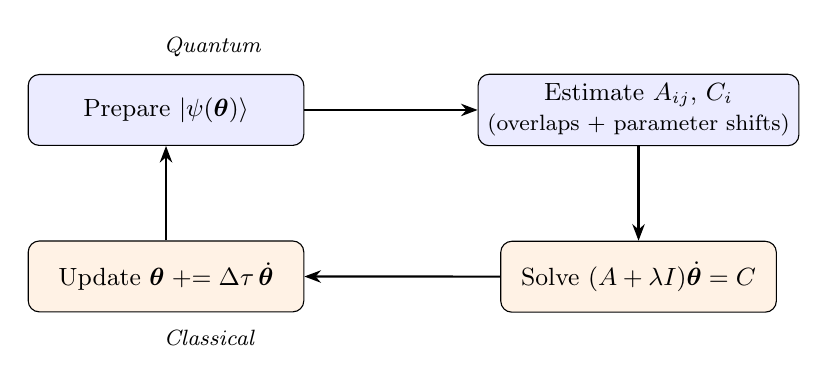
\begin{tikzpicture}[
    node distance=1.2cm and 2.2cm,
    box/.style={
      draw, rounded corners=4pt, minimum width=3.5cm,
      minimum height=0.9cm, align=center, font=\small
    },
    arrow/.style={-{Stealth[length=6pt]}, thick},
  ]
  \node[box, fill=blue!8] (prep) {Prepare $\ket{\psi(\bm{\theta})}$};
  \node[box, fill=blue!8, right=of prep] (meas)
    {Estimate $A_{ij},\,C_i$\\
     {\footnotesize (overlaps + parameter shifts)}};
  \node[box, fill=orange!10, below=of meas] (solve)
    {Solve $(A+\lambda I)\dot{\bm{\theta}} = C$};
  \node[box, fill=orange!10, below=of prep] (upd)
    {Update $\bm{\theta} \mathrel{+}= \Delta\tau\,\dot{\bm{\theta}}$};
  \draw[arrow] (prep) -- (meas);
  \draw[arrow] (meas) -- (solve);
  \draw[arrow] (solve) -- (upd);
  \draw[arrow] (upd) -- (prep);
  \node[font=\footnotesize\itshape, above=0.1cm of prep, anchor=south west,
        xshift=-0.15cm] {Quantum};
  \node[font=\footnotesize\itshape, below=0.1cm of upd, anchor=north west,
        xshift=-0.15cm] {Classical};
\end{tikzpicture}
\caption{The VQITE hybrid loop. At each step the quantum processor estimates
  the metric tensor $A$ via \cref{eq:metric_fd} and the energy gradient
  components of $C$ via the parameter-shift rule \cref{eq:param_shift}; the
  classical computer solves the linear system \cref{eq:vqite_tikhonov} and
  advances the parameters in imaginary time.}
\label{fig:vqite_loop}
\end{figure}

\subsection{Excited states by penalisation}
\label{ssec:vqite_excited}

VQITE projects onto the lowest-energy state with non-vanishing overlap with
the initial state. To target higher levels we modify the effective
Hamiltonian by adding penalty terms that suppress overlap with previously
obtained states. Concretely, if $\{\ket{\psi_k^{\star}}\}_{k=0}^{n-1}$ are
already-computed eigenstates, we replace $H$ by
\begin{equation}
  \label{eq:penalised_H}
  H_{\mathrm{eff}}
  = H + \alpha\sum_{k=0}^{n-1} \ket{\psi_k^{\star}}\bra{\psi_k^{\star}},
\end{equation}
where $\alpha$ is a positive penalty large enough to shift the energies of
the already-found states above the next eigenvalue. Running VQITE with
$H_{\mathrm{eff}}$ then converges to the next-higher eigenstate. The energy
gradient generalises to
\begin{equation}
  \label{eq:penalised_grad}
  \frac{\partial \langle H_{\mathrm{eff}}\rangle}{\partial\theta_i}
  = \frac{\partial \langle H\rangle}{\partial\theta_i}
  + 2\alpha\sum_{k}\Re\bigl[\braket{\psi_k^{\star}}{\psi}\,
                            \bra{\partial_i\psi}\psi_k^{\star}\rangle\bigr],
\end{equation}
where the overlap correction is again accessible from short fidelity
circuits. In practice $\alpha$ is chosen of the same order of magnitude as
the typical gap between adjacent eigenvalues; we use $\alpha = 10$ in
inverse-femtometre units throughout this thesis.

The combination of VQITE for the ground state with iterated penalisation
provides access to a sequence of eigenpairs without ever requiring the
diagonalisation of an exponentially large matrix on a classical computer.
The cost is a sequence of linear systems of size at most $p = 3$, an
imaginary-time integration with $O(50)$ steps per state, and a number of
small overlap circuits scaling polynomially with the number of states
targeted.


% ──────────────────────────────────────────────────────────────────
\section{Trotter--Taylor Imaginary-Time Evolution}
\label{sec:ttite}

The two methods discussed so far---VQE in \cref{sec:vqe} and VQITE in
\cref{sec:vqite}---share a common strategy: a parameterised ansatz approximates
the target state, and a classical optimiser navigates the parameter space.
This restricts the accuracy to the expressibility of the chosen ansatz. The
Trotter--Taylor Imaginary-Time Evolution (TTITE) scheme of Yi et
al.~\cite{yi2025}, by contrast, simulates the imaginary-time propagator
$e^{-H\tau}$ directly on the quantum register, without ever fitting parameters.
The price is a probabilistic structure: at each step an ancilla measurement
must yield a particular outcome, and the algorithm proceeds only when it
does. This section develops the construction in stages, applying it
throughout to the channel Hamiltonians of
\cref{eq:H_1S0,eq:H_3S1,eq:H_1P1}.

\subsection{Strategy: implement the propagator directly}
\label{ssec:ttite_strategy}

The starting point is again the eigenstate-projection property of imaginary
time \cref{eq:ite_ground_state}. We seek a unitary protocol that, given the
initial state $\ket{\psi(0)}$ on the work register, returns
\(
  \ket{\psi(\tau)} \propto e^{-H\tau}\ket{\psi(0)}
\)
to controllable accuracy. Two obstacles must be overcome.

The first obstacle is the non-unitarity of the propagator
$e^{-H\tau}$. We resolve it by writing each elementary factor of a
Trotter-decomposed propagator as a linear combination of two unitaries; such
``LCU'' operators admit a probabilistic implementation via an ancilla.

The second obstacle is that the Hamiltonian is a \emph{sum} of Pauli
strings, and exponentials of a sum cannot generally be separated. We
resolve it through the Trotter formula, which decomposes
$e^{-H\Delta\tau}$ into a product of exponentials of individual Pauli
strings, each of which is straightforward to handle.

We now make each of these steps precise.

\subsection{Trotter decomposition}
\label{ssec:trotter}

Let $H = \sum_{i=1}^{m} c_i\, h_i$ be the Pauli decomposition of one of the
channel Hamiltonians, with $c_i\in\mathbb{R}$ and each $h_i$ a Pauli string
satisfying $h_i^{2} = I$. The first-order \emph{Trotter
formula}~\cite{trotter1959,suzuki1976} approximates the imaginary-time
propagator for a small step $\Delta\tau$ as
\begin{equation}
  \label{eq:trotter}
  e^{-H\,\Delta\tau}
  = \prod_{i=1}^{m} e^{-c_i\,h_i\,\Delta\tau}
  + O\!\bigl((\Delta\tau)^{2}\bigr),
\end{equation}
with leading error proportional to the commutators $[h_i, h_j]$. To evolve
over a total imaginary time $\tau$ we apply $L = \tau/\Delta\tau$ such
Trotter steps in succession, accumulating an overall error of order
$\tau\,\Delta\tau$. Higher-order symmetric (Suzuki) schemes reduce this
error to $O(\Delta\tau^{2k+1})$ for stage-$2k$ formulas, at the cost of
more elementary exponentials per
step~\cite{suzuki1976}; for the small Hamiltonians of this work the
first-order formula \cref{eq:trotter} is already accurate enough.

\subsection{Taylor expansion of a single Trotter step}
\label{ssec:taylor_step}

Each factor $e^{-c\,h\,\Delta\tau}$ in \cref{eq:trotter} is the exponential
of an Hermitian operator whose square is the identity, $h^{2} = I$. This
property gives a remarkably simple closed form. Expanding the exponential
as a power series and separating even and odd powers,
\begin{align}
  \label{eq:taylor_series}
  e^{-c\,h\,\Delta\tau}
  &= \sum_{j=0}^{\infty} \frac{(-c\,\Delta\tau)^{j}}{j!}\,h^{j}\\
  &= \biggl(\sum_{j\text{ even}} \frac{(-c\,\Delta\tau)^{j}}{j!}\biggr)\,I
   + \biggl(\sum_{j\text{ odd}}  \frac{(-c\,\Delta\tau)^{j}}{j!}\biggr)\,h
   = \cosh(c\,\Delta\tau)\,I - \sinh(c\,\Delta\tau)\,h,
  \label{eq:closed_form}
\end{align}
where we used $h^{2k} = I$ and $h^{2k+1} = h$. The single Trotter step is
therefore exactly a linear combination of two unitaries: the identity and
$h$ itself. Truncating the series at finite order $R$,
\begin{equation}
  \label{eq:taylor_truncation}
  T^{(R)}(c\,\Delta\tau)
  \;\equiv\; \alpha\,I + \beta\,h,
  \qquad
  \alpha = \sum_{\substack{j=0\\j\text{ even}}}^{R}\!\frac{(-c\,\Delta\tau)^{j}}{j!},
  \qquad
  \beta  = \sum_{\substack{j=1\\j\text{ odd}}}^{R}\!\frac{(-c\,\Delta\tau)^{j}}{j!},
\end{equation}
incurs a Taylor error of order $(\Delta\tau)^{R+1}$, which for
$R = 4$ or higher is negligible compared to the Trotter error
$O(\Delta\tau^{2})$ in \cref{eq:trotter}. The truncation is convenient
because it makes $\alpha$ and $\beta$ polynomials in $\Delta\tau$, slightly
simpler than $\cosh$ and $\sinh$.

\begin{remark}
The closed form \cref{eq:closed_form} shows that the Taylor truncation is
in fact \emph{not necessary} for correctness; one could simply use
$\alpha = \cosh(c\,\Delta\tau)$ and $\beta = -\sinh(c\,\Delta\tau)$. The
finite-order form \cref{eq:taylor_truncation} matches the construction of
Yi et al.~\cite{yi2025} and makes the analysis of the LCU success probability
slightly more uniform across different Hamiltonians, but the algorithm
itself is unchanged.
\end{remark}

\subsection{Linear-combination-of-unitaries (LCU) implementation}
\label{ssec:lcu}

The operator $\alpha I + \beta h$ in \cref{eq:taylor_truncation} is a
non-unitary linear combination of two unitaries. Operators of this form
admit a celebrated probabilistic implementation, the LCU
construction~\cite{childs2012}, which uses a single ancillary qubit. We
derive it explicitly here.

Augment the work register with one ancilla qubit, initially in $\ket{0}$.
The combined state is $\ket{0}\otimes\ket{\psi}$. The LCU circuit applies
the following three operations.

\paragraph{(i) Ancilla preparation.}
Apply $R_y(\vartheta)$ to the ancilla with
\begin{equation}
  \label{eq:lcu_angle}
  \vartheta = 2\atantwo(\beta,\alpha),
\end{equation}
so that
\(
  R_y(\vartheta)\ket{0}
  = \cos(\vartheta/2)\ket{0} + \sin(\vartheta/2)\ket{1}
  = (\alpha\ket{0} + \beta\ket{1})/\sqrt{\alpha^{2}+\beta^{2}}.
\)
The combined state is then
\begin{equation}
  \label{eq:lcu_state1}
  \ket{\phi_1} = \frac{1}{\sqrt{\alpha^{2}+\beta^{2}}}
                 \bigl(\alpha\ket{0} + \beta\ket{1}\bigr)\otimes\ket{\psi}.
\end{equation}

\paragraph{(ii) Controlled application of $h$.}
Apply the controlled unitary
\(
  CU = \ket{0}\bra{0}\otimes I + \ket{1}\bra{1}\otimes h,
\)
which acts as the identity if the ancilla is $\ket{0}$ and as $h$ if it is
$\ket{1}$. Since $h$ is a Pauli string of length $n$, the controlled gate
decomposes into $n$ elementary controlled-Pauli gates acting on the work
qubits. After this step,
\begin{equation}
  \label{eq:lcu_state2}
  \ket{\phi_2}
  = \frac{1}{\sqrt{\alpha^{2}+\beta^{2}}}
    \bigl(\alpha\ket{0}\otimes\ket{\psi}
        + \beta\ket{1}\otimes h\ket{\psi}\bigr).
\end{equation}

\paragraph{(iii) Hadamard and measurement on the ancilla.}
Apply a Hadamard gate to the ancilla and then measure it in the
computational basis. Using $H\ket{0} = (\ket{0}+\ket{1})/\sqrt{2}$,
$H\ket{1} = (\ket{0}-\ket{1})/\sqrt{2}$, the state just before measurement
is
\begin{equation}
  \label{eq:lcu_state3}
  \ket{\phi_3}
  = \frac{1}{\sqrt{2(\alpha^{2}+\beta^{2})}}
    \Bigl(\ket{0}\otimes(\alpha I + \beta h)\ket{\psi}
        + \ket{1}\otimes(\alpha I - \beta h)\ket{\psi}\Bigr).
\end{equation}
A measurement outcome of $0$ on the ancilla projects the work register onto
the (unnormalised) state $(\alpha I + \beta h)\ket{\psi}$. After
renormalisation this is precisely the desired truncated Trotter step.

The probability of measuring $\ket{0}$ on the ancilla,
\begin{equation}
  \label{eq:lcu_success}
  P_{\mathrm{s}} =
  \frac{\bigl\|(\alpha I + \beta h)\ket{\psi}\bigr\|^{2}}
       {2(\alpha^{2} + \beta^{2})},
\end{equation}
sets the cost of the protocol: if the measurement returns $\ket{1}$ the
work state has been corrupted and the segment must be restarted from
$\ket{\psi}$. For small $\Delta\tau$ one has $\alpha \approx 1$ and
$\beta \approx -c\Delta\tau$, so $P_{\mathrm{s}}\approx 1/2$; the protocol
is therefore efficient at small step sizes.

\Cref{fig:lcu_circuit} summarises the LCU circuit graphically.

\begin{figure}[htbp]
\centering
\begin{quantikz}[column sep=10pt]
  \lstick[1]{anc.\ $\ket{0}$} & \gate{R_y(\vartheta)} & \ctrl{1}     & \gate{H}    & \meter{} \\
  \lstick[1]{$\ket{\psi}$}    & \qw                   & \gate{h}     & \qw         & \rstick{$\frac{(\alpha I + \beta h)\ket{\psi}}{\bigl\|(\alpha I + \beta h)\ket{\psi}\bigr\|}$ on $\ket{0}_{\mathrm{anc}}$} \qw
\end{quantikz}
\caption{LCU circuit implementing one truncated Trotter step
  $T^{(R)}(c\,\Delta\tau) = \alpha I + \beta h$ on the work register
  $\ket{\psi}$. The ancilla is rotated by an angle
  $\vartheta = 2\atantwo(\beta,\alpha)$, a controlled application of the
  Pauli string $h$ entangles ancilla and work, a Hadamard interferes the
  two LCU branches, and a measurement on the ancilla post-selects the
  desired branch. The work register collapses to the (renormalised)
  truncated step exactly when the measurement outcome is $0$, an event of
  probability $P_{\mathrm{s}}$ given by \cref{eq:lcu_success}.}
\label{fig:lcu_circuit}
\end{figure}

\subsection{The full TTITE algorithm}
\label{ssec:ttite_full}

Composing the building blocks of
\cref{ssec:trotter,ssec:taylor_step,ssec:lcu} yields the complete TTITE
procedure, summarised in \cref{alg:ttite}.

\begin{figure}[htbp]
\centering
\fbox{\begin{minipage}{0.94\textwidth}\small
\textbf{Algorithm: TTITE.} \\[2pt]
\textit{Input:} Pauli decomposition $H = \sum_{i=1}^{m} c_i\,h_i$; initial
state $\ket{\psi_0}$; total time $\tau$; step size $\Delta\tau$; Taylor
order $R$. \\
\textit{Output:} an approximation to
$e^{-H\tau}\ket{\psi_0}/\|e^{-H\tau}\ket{\psi_0}\|$.

\begin{enumerate}\setlength{\itemsep}{2pt}
  \item Set $L = \lceil\tau/\Delta\tau\rceil$ and $\ket{\psi}\leftarrow\ket{\psi_0}$.
  \item Repeat $L$ times:
  \begin{enumerate}
    \item For $i = 1,\ldots,m$:
    \begin{enumerate}
      \item Compute the Taylor coefficients $\alpha,\beta$ from
        \cref{eq:taylor_truncation} with $c=c_i$ and $h=h_i$.
      \item Build the LCU circuit of \cref{fig:lcu_circuit} with angle
        \cref{eq:lcu_angle} and controlled-Pauli string $h_i$.
      \item Execute the circuit on $\ket{0}_{\mathrm{anc}}\otimes\ket{\psi}$;
        on outcome $0$ update $\ket{\psi}$ with the (renormalised) post-selected
        state; on outcome $1$ \emph{restart} the current Trotter step.
    \end{enumerate}
  \end{enumerate}
  \item Return $\ket{\psi}$.
\end{enumerate}
\end{minipage}}
\caption{Pseudocode for the TTITE algorithm. Each Trotter step requires $m$
  successful LCU post-selections; the per-segment success probability is
  given by \cref{eq:segment_success}.}
\label{alg:ttite}
\end{figure}

The algorithm is generic in the Hamiltonian: it uses only the Pauli
decomposition produced in \cref{sec:encoding} and the (small) number of
qubits required by that encoding. In this work we apply it to the channel
Hamiltonians in the direct encoding (two work qubits plus one ancilla,
i.e.\ three qubits in total).

\begin{remark}[Originally on $\mathrm{H}_2$ and Heisenberg models]
The algorithm was introduced and demonstrated by Yi et al.~\cite{yi2025} on
the molecular hydrogen ($\mathrm{H}_{2}$) Hamiltonian and on
one-dimensional Heisenberg spin chains. Because the procedure depends only
on the Pauli decomposition of the Hamiltonian, it transfers without
modification to the channel Hamiltonians of \cref{eq:H_1S0,eq:H_3S1,eq:H_1P1};
we will benchmark its convergence on those Hamiltonians in subsequent
chapters.
\end{remark}

\subsection{Success probability and resource cost}
\label{ssec:ttite_resources}

Each Trotter step requires $m$ LCU circuits to succeed (one per Pauli term),
so the segment-level success probability factorises:
\begin{equation}
  \label{eq:segment_success}
  P_{\mathrm{seg}} = \prod_{i=1}^{m} P_{\mathrm{s},i},
\end{equation}
with $P_{\mathrm{s},i}$ given by \cref{eq:lcu_success}. For small
$\Delta\tau$ each individual factor approaches $1/2$, so the per-segment
probability decays exponentially in the number of Pauli terms. Two
observations soften this otherwise daunting cost.

First, Yi et al.~\cite{yi2025} prove that the success probability is
\emph{monotonically non-decreasing} in the imaginary-time step: as the
state approaches the ground state, applying $H - E_0$ becomes
quasi-tangential to it, which inflates the success probabilities
$P_{\mathrm{s},i}$. Concretely, with $\tau_\ell = \ell\,\Delta\tau$ denoting
the cumulative imaginary time after the $\ell$-th segment,
\begin{equation}
  \label{eq:monotone_success}
  P_{\mathrm{seg}}(\tau_1) \;\leq\;
  P_{\mathrm{seg}}(\tau_2) \;\leq\;
  \cdots \;\leq\;
  P_{\mathrm{seg}}(\tau_L),
\end{equation}
so the algorithm becomes \emph{more} efficient as it converges.

Second, the failure probability $1 - P_{\mathrm{s},i}$ can be amplified
toward zero by amplitude
amplification, at a cost of additional ancillas and depth. We do not employ
amplitude amplification in this work, instead relying on the simpler
repeat-until-success strategy described in
\cref{alg:ttite}. For the two-qubit channel Hamiltonians considered here
the per-segment cost is at most a small multiplicative overhead, and the
algorithm remains practical for the imaginary times required to reach the
ground state.

The overall picture is therefore the following. TTITE bypasses the
parameter-space optimisation of VQE and VQITE by implementing the
imaginary-time propagator more or less directly on the device, at the price
of an ancilla and a post-selection step per Pauli term. Its accuracy is
controlled by two parameters, $\Delta\tau$ and $R$, and is unaffected by
ansatz expressibility. We will see in the next chapters how the three
algorithms compare on the same channel Hamiltonians.


% ──────────────────────────────────────────────────────────────────
\section{Transition Amplitudes}
\label{sec:transitions}

The algorithms in the previous sections produce eigenstates of the
individual channel Hamiltonians. Most experimentally accessible observables,
however, involve \emph{matrix elements} of an operator between two such
eigenstates---typically a transition operator inducing a radiative decay
from a heavier state to a lighter one. In this section we develop the
quantum-circuit techniques required to evaluate the two transition types
relevant to charmonium spectroscopy: the magnetic-dipole (M1) transitions
between spin partners, and the electric-dipole (E1) transitions that
change the orbital angular momentum.

\subsection{Physical motivation}
\label{ssec:transitions_physics}

In the multipole expansion of the electromagnetic interaction of a
quark--antiquark system, the leading single-photon transitions are
classified by their selection rules~\cite{brambilla2011}:
\begin{itemize}\setlength{\itemsep}{2pt}
  \item \emph{M1 transitions} flip the total spin without changing the
    orbital angular momentum ($\Delta S = 1$, $\Delta L = 0$). In the
    non-relativistic limit the amplitude reduces to a wavefunction overlap
    between the two spin partners, scaled by a numerical prefactor.
  \item \emph{E1 transitions} change the orbital angular momentum by one
    unit without altering the spin ($\Delta S = 0$, $\Delta L = 1$). The
    amplitude is proportional to the radial matrix element of the
    position operator, $\bra{\psi_f}r\ket{\psi_i}$.
\end{itemize}
The two paradigmatic examples for charmonium are
$J/\psi \to \eta_c\,\gamma$ (M1) and $h_c \to \eta_c\,\gamma$ (E1).
Computing their amplitudes therefore amounts to evaluating, respectively,
the overlap $\braket{\psi_f^{({}^1S_0)}}{\psi_i^{({}^3S_1)}}$ and the matrix
element $\bra{\psi_f^{({}^1S_0)}}r\ket{\psi_i^{({}^1P_1)}}$, where the
states are the eigenvectors produced by VQE, VQITE, or TTITE.

\subsection{M1 transitions: state overlaps}
\label{ssec:m1}

In the non-relativistic limit, the M1 transition amplitude between two
states differing only in spin reduces to an overlap of their spatial
wavefunctions,
\begin{equation}
  \label{eq:m1_amplitude}
  |\mathcal{M}_{\mathrm{M1}}|^{2} \;\propto\;
  \bigl|\braket{\psi_f^{\mathrm{spatial}}}{\psi_i^{\mathrm{spatial}}}\bigr|^{2}.
\end{equation}
The two states are eigenvectors of different channel Hamiltonians
(${}^1S_0$ and ${}^3S_1$) but live in the same HO basis, so their overlap
is well-defined as a four-dimensional inner product of real coefficient
vectors. Three quantum-circuit techniques are available to estimate this
overlap.

\paragraph{Inverse-ansatz protocol.}
If the two ansatz unitaries $U_i = U(\bm{\theta}_i^{\star})$ and
$U_f = U(\bm{\theta}_f^{\star})$ have been determined---e.g., as the output of
two VQE or VQITE runs---then the overlap can be read off from the
all-zero outcome of the circuit $U_f^{\dagger} U_i\ket{0}^{\otimes n}$. Indeed,
\begin{equation}
  \label{eq:inverse_ansatz}
  \mathrm{Prob}\bigl(\text{all zeros}\bigr) =
    \bigl|\bra{0}^{\otimes n}\,U_f^{\dagger} U_i\,\ket{0}^{\otimes n}\bigr|^{2}
  = \bigl|\braket{\psi_f}{\psi_i}\bigr|^{2}.
\end{equation}
This protocol requires no additional qubits, only an inverse-ansatz
sub-circuit, and is the most economical method available when both ansatz
unitaries can be efficiently implemented.

\paragraph{Swap test.}
A more general protocol, applicable when $\ket{\psi_i}$ and $\ket{\psi_f}$
are prepared independently on two copies of the work register, is the swap
test~\cite{nielsen2010}. Adding one ancilla initialised in $\ket{0}$, the
circuit
\begin{equation}
  \label{eq:swap_test}
  \ket{0}\otimes\ket{\psi_i}\otimes\ket{\psi_f}
  \;\xrightarrow{H_{\mathrm{anc}}}\;
  \cdots
  \;\xrightarrow{\mathrm{CSWAP}}\;
  \cdots
  \;\xrightarrow{H_{\mathrm{anc}}}\;
  \ket{\phi}
\end{equation}
yields an ancilla-zero probability
\(
  \mathrm{Prob}(0_{\mathrm{anc}})
   = \tfrac{1}{2}\bigl(1 + |\braket{\psi_f}{\psi_i}|^{2}\bigr),
\)
from which the overlap squared is recovered as
$2\,\mathrm{Prob}(0_{\mathrm{anc}}) - 1$. The swap test is more demanding in
qubits ($2n + 1$ total) and gates ($n$ controlled-SWAPs), but does not
require explicit knowledge of either ansatz unitary, only the ability to
prepare both states on demand. The corresponding circuit is shown in
\cref{fig:swap_test}.

\begin{figure}[htbp]
\centering
\begin{quantikz}[column sep=10pt]
  \lstick{$\ket{0}_{\mathrm{anc}}$} & \gate{H} & \ctrl{1}  & \gate{H} & \meter{} \\
  \lstick{$\ket{\psi_i}$}           & \qw      & \swap{1}  & \qw      & \qw \\
  \lstick{$\ket{\psi_f}$}           & \qw      & \targX{}  & \qw      & \qw
\end{quantikz}
\caption{Swap test for the absolute overlap between two ansatz states
  $\ket{\psi_i}$ and $\ket{\psi_f}$. The Hadamard--CSWAP--Hadamard sandwich
  interferes the swapped and unswapped configurations of the work registers;
  the ancilla-zero probability is
  $(1 + |\braket{\psi_f}{\psi_i}|^{2})/2$. The CSWAP gate acts as a
  controlled exchange of the two work registers.}
\label{fig:swap_test}
\end{figure}

\paragraph{Hadamard test.}
When the overlap itself rather than its absolute value is required---e.g.\
for complex amplitudes or for matrix elements of non-unitary
operators---the Hadamard test~\cite{nielsen2010} is more appropriate. We
discuss it in the context of E1 transitions in the next subsection.

\subsection{E1 transitions: matrix elements of the radial operator}
\label{ssec:e1}

For E1 transitions the relevant matrix element is the radial dipole
amplitude $\bra{\psi_f}r\ket{\psi_i}$, where $\ket{\psi_i}$ and
$\ket{\psi_f}$ are eigenstates of the initial- and final-state channels.
In the HO basis the radial operator is an $N\times N$ matrix
$R_{mk} = \bra{\phi_{m\,\ell_f}} r \ket{\phi_{k\,\ell_i}}$ which, like the
Hamiltonian, can be evaluated in closed form. Using the same techniques
that produced \cref{eq:linear_matrix}, one obtains, for the
$P\to S$ case ($\ell_i = 1, \ell_f = 0$) and $N = 4$, the explicit
matrix~\cite{woloshyn2023}
\begin{equation}
  \label{eq:r_matrix}
  R \;=\;
  \begin{pmatrix}
    0.5775 & -0.4715 & 0      & 0      \\
    0      &  0.8821 & -0.6668 & 0     \\
    0      &  0      &  0.8821 & -0.8167\\
    0      &  0      &  0      &  1.0002
  \end{pmatrix}
  \quad \text{(units of fm)}.
\end{equation}
The amplitude is then
\begin{equation}
  \label{eq:e1_amplitude}
  \bra{\psi_f}r\ket{\psi_i} = \mathbf{c}_f^{\!\top} R\,\mathbf{c}_i,
\end{equation}
where $\mathbf{c}_i$ and $\mathbf{c}_f$ are the real coefficient vectors of
$\ket{\psi_i}$ and $\ket{\psi_f}$ in the HO basis.

\begin{remark}[Errata]
Woloshyn's Eq.~(13) reports the $(2,2)$ element of $R$ as $5.4382$, which
is in fact the numerical value of an entry in the ${}^1S_0$ Hamiltonian
matrix \cref{eq:H_1S0}; the correct value, consistent with the
monotonically growing radial-element pattern, is $0.8821$, as used in
\cref{eq:r_matrix}. This is one of two copy-paste errata noted in
\cref{ssec:matrices,ssec:e1}.
\end{remark}

To extract $\bra{\psi_f}r\ket{\psi_i}$ on a quantum device, we first Pauli-
decompose the operator $R$ on the work register (analogously to
\cref{ssec:pauli_decomp}). The matrix element then reduces to a sum of
terms of the form $\bra{\psi_f}P\ket{\psi_i}$ for Pauli strings $P$. Each
such term can be estimated by the \emph{Hadamard test}: with one ancilla
qubit prepared in $\ket{0}$, the circuit shown in
\cref{fig:hadamard_test} yields an ancilla-zero probability
\begin{equation}
  \label{eq:hadamard_test}
  \mathrm{Prob}(0_{\mathrm{anc}})
  = \frac{1 + \Re\,\bra{\psi_f}P\ket{\psi_i}}{2},
\end{equation}
from which the real part of the matrix element is obtained as
$2\,\mathrm{Prob}(0_{\mathrm{anc}}) - 1$. Replacing the leading Hadamard
on the ancilla by a $S^{\dagger} H$ rotation yields, by the same algebra,
the imaginary part of the matrix element. For real-symmetric problems such
as the channel Hamiltonians considered here, only the real part is needed.

\begin{figure}[htbp]
\centering
\begin{quantikz}[column sep=10pt]
  \lstick{$\ket{0}_{\mathrm{anc}}$} & \gate{H} & \ctrl{1}     & \gate{H} & \meter{} \\
  \lstick{$\ket{\psi_i}$}           & \gate{U_{f\leftarrow i}^{\dagger}\,P} & \qw & \qw & \qw
\end{quantikz}
\caption{Hadamard test for the matrix element $\bra{\psi_f}P\ket{\psi_i}$.
  Conditioned on the ancilla, the work register is rotated by an operator
  whose expectation value coincides with the desired matrix element. The
  ancilla-zero probability is $(1 + \Re\bra{\psi_f}P\ket{\psi_i})/2$.
  Replacing the first Hadamard by $S^{\dagger}H$ gives the imaginary part.}
\label{fig:hadamard_test}
\end{figure}

Putting the pieces together, the E1 transition amplitude is computed as a
weighted sum of Hadamard tests, one per Pauli string in the decomposition
of $R$:
\begin{equation}
  \label{eq:e1_decomposed}
  \bra{\psi_f}r\ket{\psi_i}
  = \sum_k r_k\,\bra{\psi_f}P_k\ket{\psi_i},
\end{equation}
where $r_k$ are the Pauli coefficients of $R$ obtained from
\cref{eq:pauli_sum}. The number of measurements scales with the number of
Pauli strings, which for the $4\times 4$ matrix \cref{eq:r_matrix} is at
most $4^{2} = 16$ and typically much smaller after symmetry-based
truncation.

With this construction, the same quantum-algorithmic framework that yields
energies also yields the matrix elements needed for radiative transitions,
allowing a direct comparison with experimental decay widths and lifetimes
once eigenstates have been obtained.


% ──────────────────────────────────────────────────────────────────
\section{Summary}
\label{sec:framework-summary}

The framework developed in this chapter equips us with everything needed to
run the three algorithms on the charmonium channels of interest. The
Hamiltonian construction of \cref{sec:hamiltonian} produces three
$4\times 4$ real-symmetric matrices encoding the ${}^1S_0$, ${}^3S_1$, and
${}^1P_1$ physics; the encodings of \cref{sec:encoding} translate each into a
sum of Pauli strings on either two or four qubits; the algorithms of
\cref{sec:vqe,sec:vqite,sec:ttite} provide three independent routes to the
spectrum of those operators; and the transition machinery of
\cref{sec:transitions} extends the algorithmic toolkit to observable
amplitudes.

The three algorithms differ in significant ways, summarised in
\cref{tab:algo_compare}. VQE replaces the diagonalisation of the
Hamiltonian by a classical optimisation over a parameterised state; its
quality is set by the expressibility of the ansatz and by the convergence of
the classical optimiser. VQITE retains a parameterised state but evolves it
in imaginary time according to the McLachlan principle, trading one
optimisation problem for a sequence of small linear systems. TTITE
sidesteps parameterisation entirely, implementing the imaginary-time
propagator probabilistically through LCU circuits; its cost migrates from
classical optimisation to ancilla overhead and post-selection.

\begin{table}[htbp]
\centering
\caption{Side-by-side comparison of the three algorithms developed in this
  chapter, as applied to the channel Hamiltonians of
  \cref{eq:H_1S0,eq:H_3S1,eq:H_1P1}. The ``classical workload'' refers to
  the classical computation per iteration; the ``quantum workload'' refers
  to the number and depth of circuits executed per iteration. All three
  algorithms apply to either qubit encoding of \cref{sec:encoding}.}
\label{tab:algo_compare}
\renewcommand{\arraystretch}{1.15}
\begin{tabular}{p{0.22\textwidth}p{0.24\textwidth}p{0.24\textwidth}p{0.24\textwidth}}
\toprule
                 & VQE                            & VQITE                          & TTITE                          \\
\midrule
What is updated  & ansatz parameters              & ansatz parameters              & work-register state itself     \\[2pt]
What is optimised& energy expectation value       & McLachlan residual norm        & --- (no parameters)            \\[2pt]
Classical workload & gradient-free optimiser      & small linear-system solves     & track ancilla outcomes         \\[2pt]
Quantum workload   & $\sim m$ circuits / iter.    & $\sim m + p^{2}$ circuits / step & $\sim m$ LCU circuits / step \\[2pt]
Excited states     & orthogonality constraints    & state-overlap penalties        & not directly supported         \\[2pt]
Ancilla qubits     & none                         & none                           & one per Trotter step           \\[2pt]
Dominant error     & ansatz expressibility        & ansatz + Trotter-like step     & Trotter + Taylor + finite shots\\
\bottomrule
\end{tabular}
\end{table}

A few qualitative consequences of \cref{tab:algo_compare} deserve emphasis.
First, VQE and VQITE share the same parameterised ansatz, so their
expressibility limits coincide; differences in their numerical performance
on the channel Hamiltonians will therefore reflect the relative merits of
direct optimisation versus geometry-respecting imaginary-time descent.
Second, TTITE achieves accuracy independent of any ansatz, which is
attractive in principle but requires an ancilla qubit and at least one
controlled-Pauli string per Hamiltonian term, so its hardware cost grows
with the size of the Pauli decomposition. Third, transitions, treated in
\cref{sec:transitions}, are post-processing operations on eigenstates
produced by any of the three methods; their accuracy is therefore directly
inherited from the underlying eigenstate accuracy.

The next chapter applies all three algorithms to the channel Hamiltonians,
quantifying these trade-offs through numerical experiments with the
codebase developed alongside this thesis.


% Placeholder for future chapters
% % ══════════════════════════════════════════════════════════════════
\chapter{Results}
\label{ch:results}

This chapter reports the numerical results obtained by applying the
four computational strategies of \cref{ch:framework} to the
spin-dependent charmonium Hamiltonians of \cref{ssec:matrices}: exact
diagonalisation (classical reference), VQE in the direct (2-qubit) and
Jordan--Wigner (4-qubit) encodings, VQITE, and TTITE. We first run a
noiseless sanity check on a simulator (\cref{sec:noiseless}), then
re-execute the same protocols under depolarising noise to characterise
the resilience of each method (\cref{sec:noisy}). A brief summary
(\cref{sec:results-summary}) closes the chapter.

% ──────────────────────────────────────────────────────────────────
\section{Experimental setup}
\label{sec:results-setup}

All quantum computations run through Qiskit's
\texttt{AerSimulator}. Pauli expectation values are
estimated with $N_{\mathrm{shots}} = 8192$ shots per term; VQITE
overlaps for the metric tensor use $4\!\times\! N_{\mathrm{shots}}$. The
classical optimiser for VQE is COBYLA with a maximum of $300$
iterations. VQITE uses $40$ forward-Euler imaginary-time steps with
$\Delta\tau = 0.05$ and Tikhonov regularisation $\lambda = 10^{-3}$.
TTITE uses total imaginary time $\tau_{\mathrm{total}} = 5$ with step
$\Delta\tau = 0.02$ and Taylor order $R = 10$. The depolarising channel
of \cref{eq:depolarizing} is applied to every gate when the noisy
backend is in use; rates swept are
$p \in \{0.0, 0.005, 0.01, 0.02, 0.05\}$ with three independent repeats
per configuration. A random seed (42) makes the runs reproducible. All
energies below are reported in inverse-femtometres; multiplication by
$\hbar c = 197.326$~MeV$\cdot$fm converts to MeV.

The full implementation---including the Hamiltonian builders, the three
algorithm wrappers, the noise sweep driver, and the standalone
visualisation script that produces every figure in this chapter---is
released as open-source software at
\url{https://github.com/Lucas-Froguel/quarkonium-simulations}~\cite{froguel_quarksim},
together with all configuration files needed to reproduce the runs
reported below.

% ──────────────────────────────────────────────────────────────────
\section{Noiseless benchmark}
\label{sec:noiseless}

\subsection{Ground-state energies}
\label{ssec:noiseless-ground}

\Cref{tab:noiseless} reports the ground-state energy of each channel
obtained by each method, alongside the exact diagonalisation reference.
\Cref{fig:convergence} shows the corresponding energy convergence
traces: COBYLA iterations for VQE, imaginary-time steps for VQITE,
Trotter segments for TTITE.

\begin{table}[htbp]
\centering
\caption{Ground-state energies in the noiseless simulator
  ($p = 0$). Energies in fm$^{-1}$; absolute errors are
  $\Delta E = |E_{\mathrm{est}} - E_{\mathrm{exact}}|$. ``VQE'' uses
  the direct encoding (2 qubits); ``VQE-JW'' uses the Jordan--Wigner
  encoding (4 qubits, UCC ansatz). $\mathcal{F}$ is the fidelity with
  the exact ground state.}
\label{tab:noiseless}
\renewcommand{\arraystretch}{1.15}
\small
\begin{tabular}{llrrrr}
\toprule
Channel & Method   & $E_{\mathrm{est}}$ & $E_{\mathrm{exact}}$ & $\Delta E$  & $\mathcal{F}$ \\
\midrule
\multirow{4}{*}{${}^1S_0$}
        & VQE      & $0.452$ & $0.391$ & $0.060$ & $0.975$ \\
        & VQE-JW   & $0.419$ & $0.391$ & $0.027$ & $0.989$ \\
        & VQITE    & $0.376$ & $0.391$ & $0.016$ & $0.99995$ \\
        & TTITE    & $0.419$ & $0.391$ & $0.027$ & $0.99984$ \\
\midrule
\multirow{4}{*}{${}^3S_1$}
        & VQE      & $0.769$ & $0.752$ & $0.017$ & $0.991$ \\
        & VQE-JW   & $0.735$ & $0.752$ & $0.017$ & $0.993$ \\
        & VQITE    & $0.744$ & $0.752$ & $0.008$ & $0.99990$ \\
        & TTITE    & $0.770$ & $0.752$ & $0.018$ & $0.99989$ \\
\midrule
\multirow{4}{*}{${}^1P_1$}
        & VQE      & $2.780$ & $2.781$ & $0.001$ & $0.998$ \\
        & VQE-JW   & $2.745$ & $2.781$ & $0.036$ & $0.999$ \\
        & VQITE    & $7.416$ & $2.781$ & $4.635$ & $0.169$ \\
        & TTITE    & $2.785$ & $2.781$ & $0.003$ & $0.99998$ \\
\bottomrule
\end{tabular}
\end{table}

\begin{figure}[htbp]
\centering
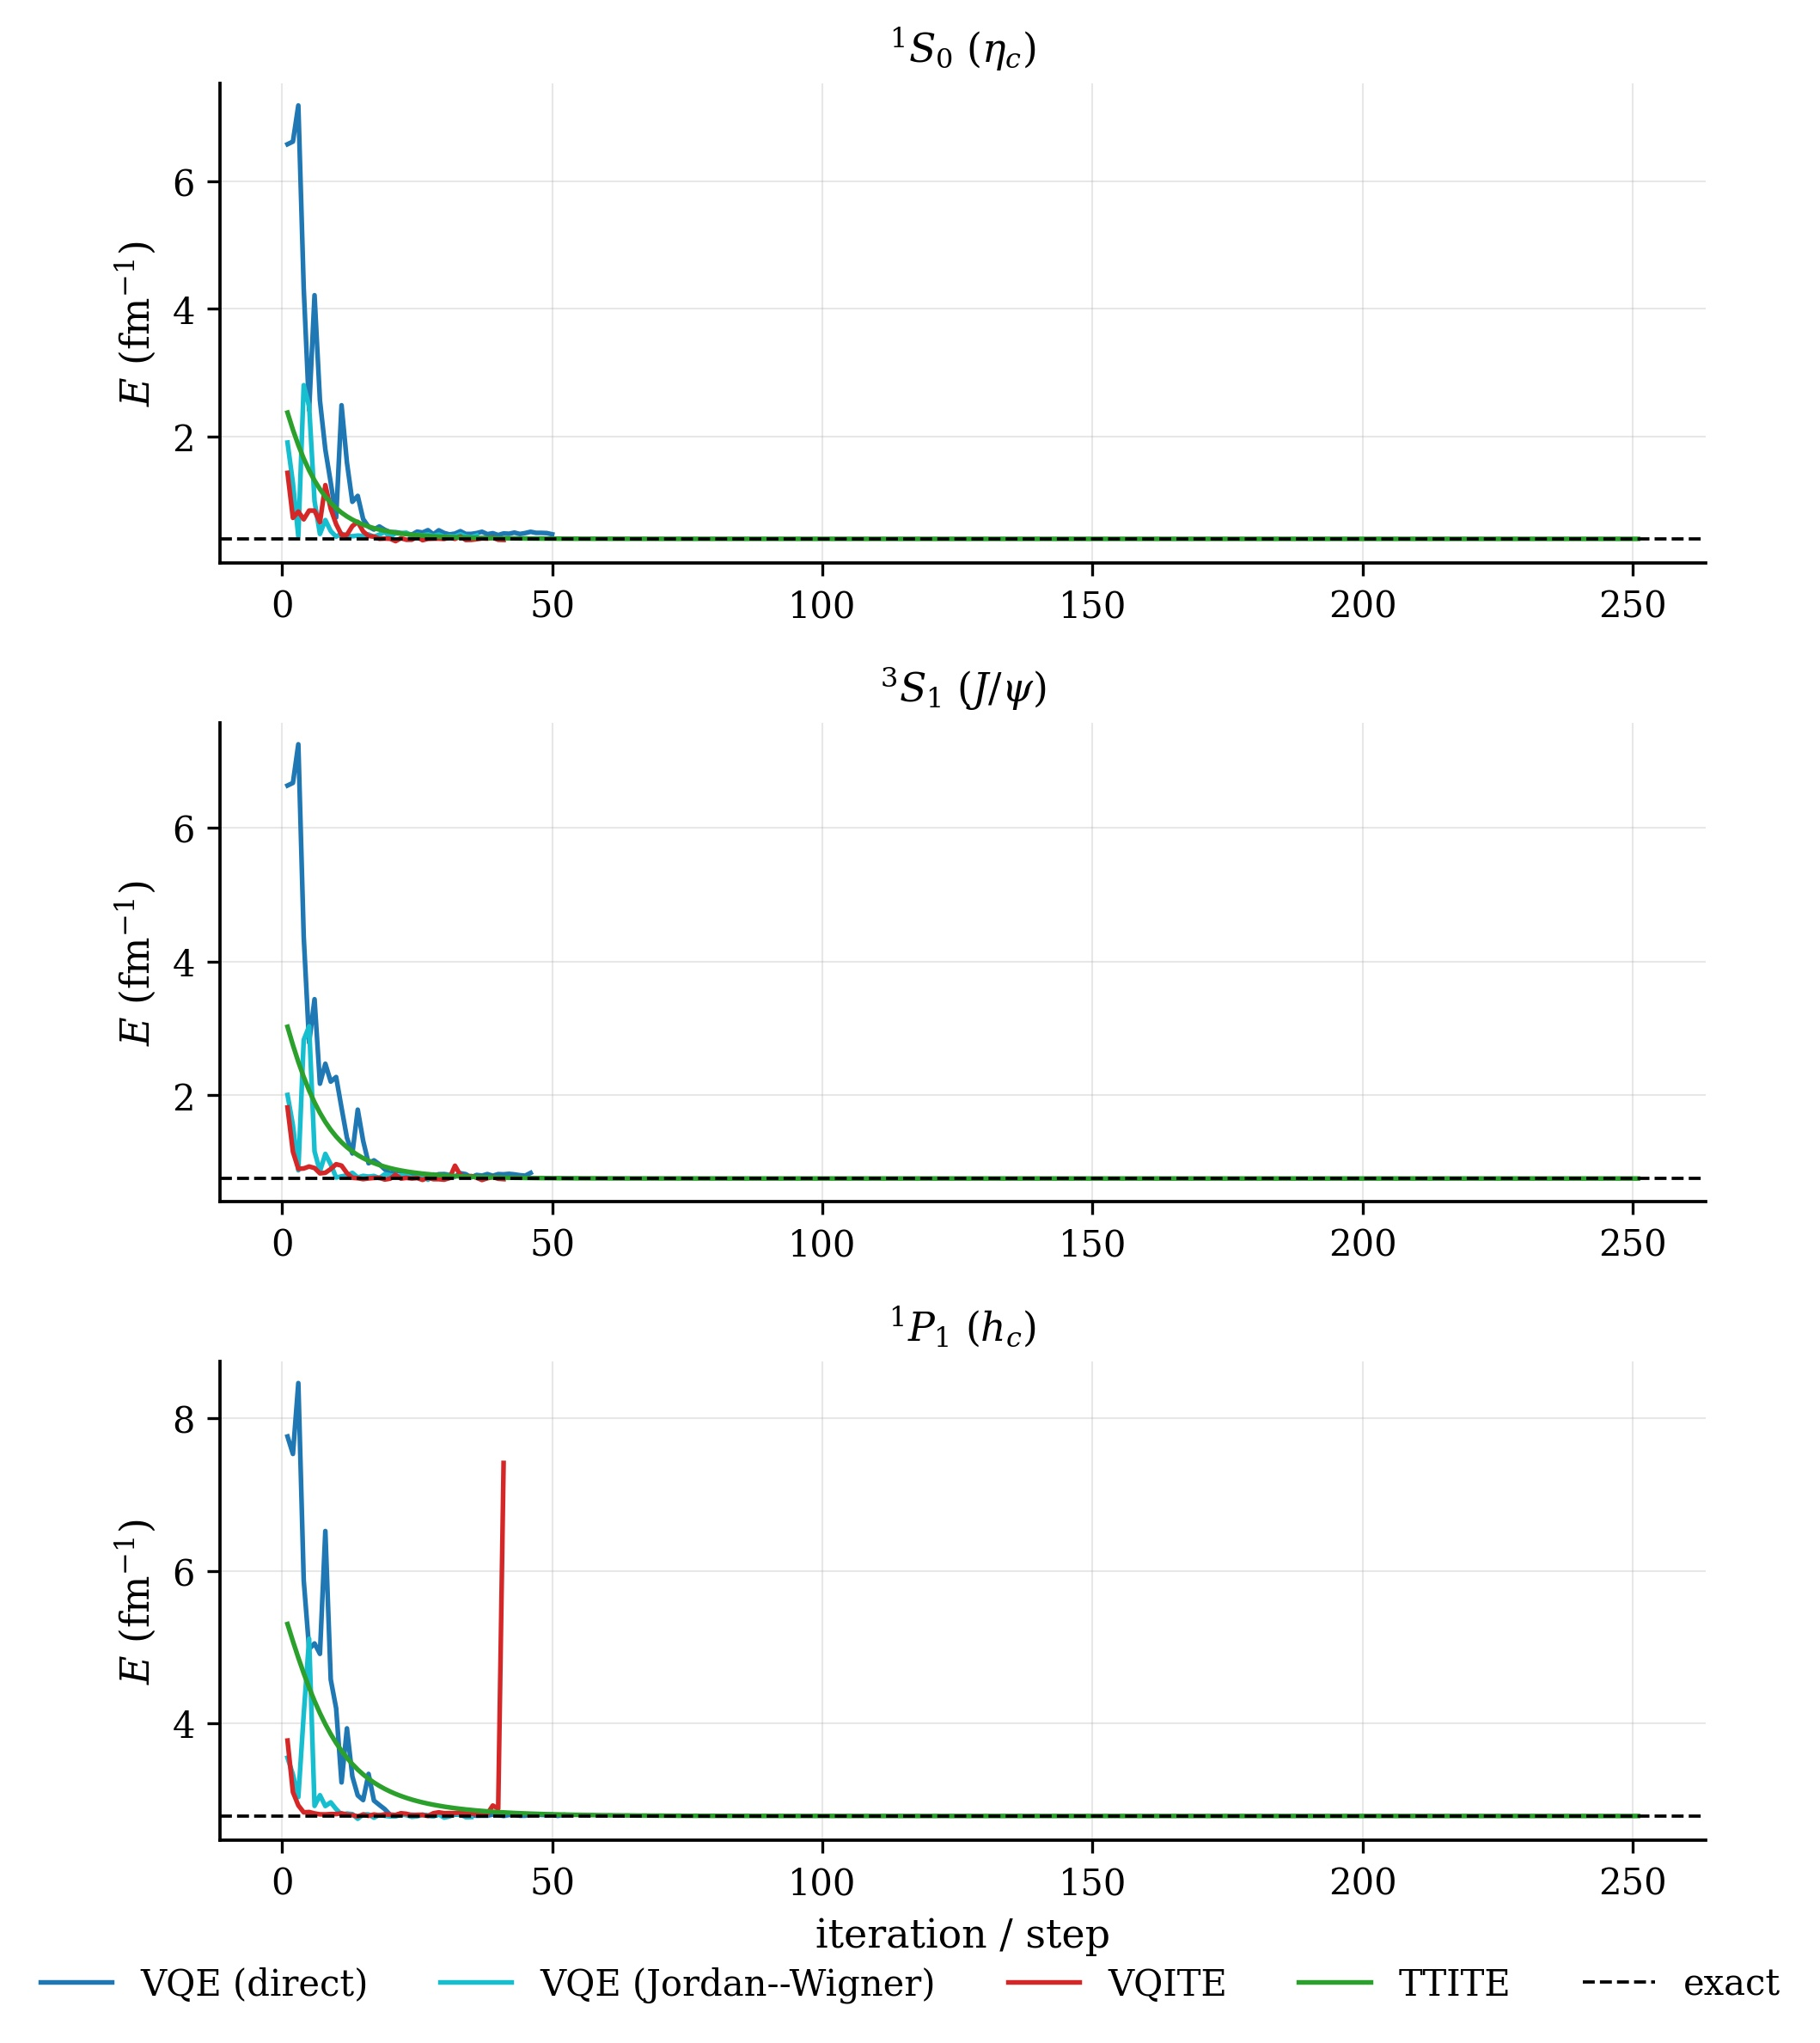
\includegraphics[width=\textwidth]{figures/convergence.jpeg}
\caption{Noiseless energy convergence on each channel. The horizontal
  dashed line marks the exact eigenvalue. The $x$-axis is the COBYLA
  iteration for VQE/VQE-JW, the imaginary-time step for VQITE, and the
  Trotter segment for TTITE.}
\label{fig:convergence}
\end{figure}

Three patterns emerge. First, TTITE consistently produces a
high-fidelity ground state (\,$\mathcal{F} \gtrsim 0.9999$ on every
channel), reflecting the fact that the algorithm does not depend on
ansatz expressibility; its $\mathcal{O}(10^{-2})$~fm$^{-1}$ energy
error is dominated by the shot-noise estimator of the final
expectation value rather than by any algorithmic bias. Second, the
two VQE variants agree to within $\sim 10^{-2}$~fm$^{-1}$ across all
channels, confirming that the Jordan--Wigner encoding faithfully
reproduces the physics encoded by the direct mapping. Third, VQITE is
the most volatile of the three: on ${}^1S_0$ and ${}^3S_1$ it
recovers the true ground state with fidelity above $0.9999$, but on
${}^1P_1$ the local McLachlan descent on the three-parameter
manifold falls into an unphysical region (final energy $7.42$, well
above any low-lying eigenvalue, fidelity $\sim 0.17$). The failure is
a known sensitivity of VQITE to the initial parameter point and to
shot noise on the quantum metric estimate; VQE on the same ansatz is
not similarly trapped because COBYLA samples a trust region and can
escape such basins.

\subsection{Ground-state error summary}
\label{ssec:noiseless-summary}

\Cref{fig:energy_summary} collects the absolute errors of
\cref{tab:noiseless} into a single bar chart, separating the
$\sim 10^{-3}$ accuracy of TTITE from the $\sim 10^{-2}$ ansatz-limited
accuracy of the variational methods.

\begin{figure}[htbp]
\centering
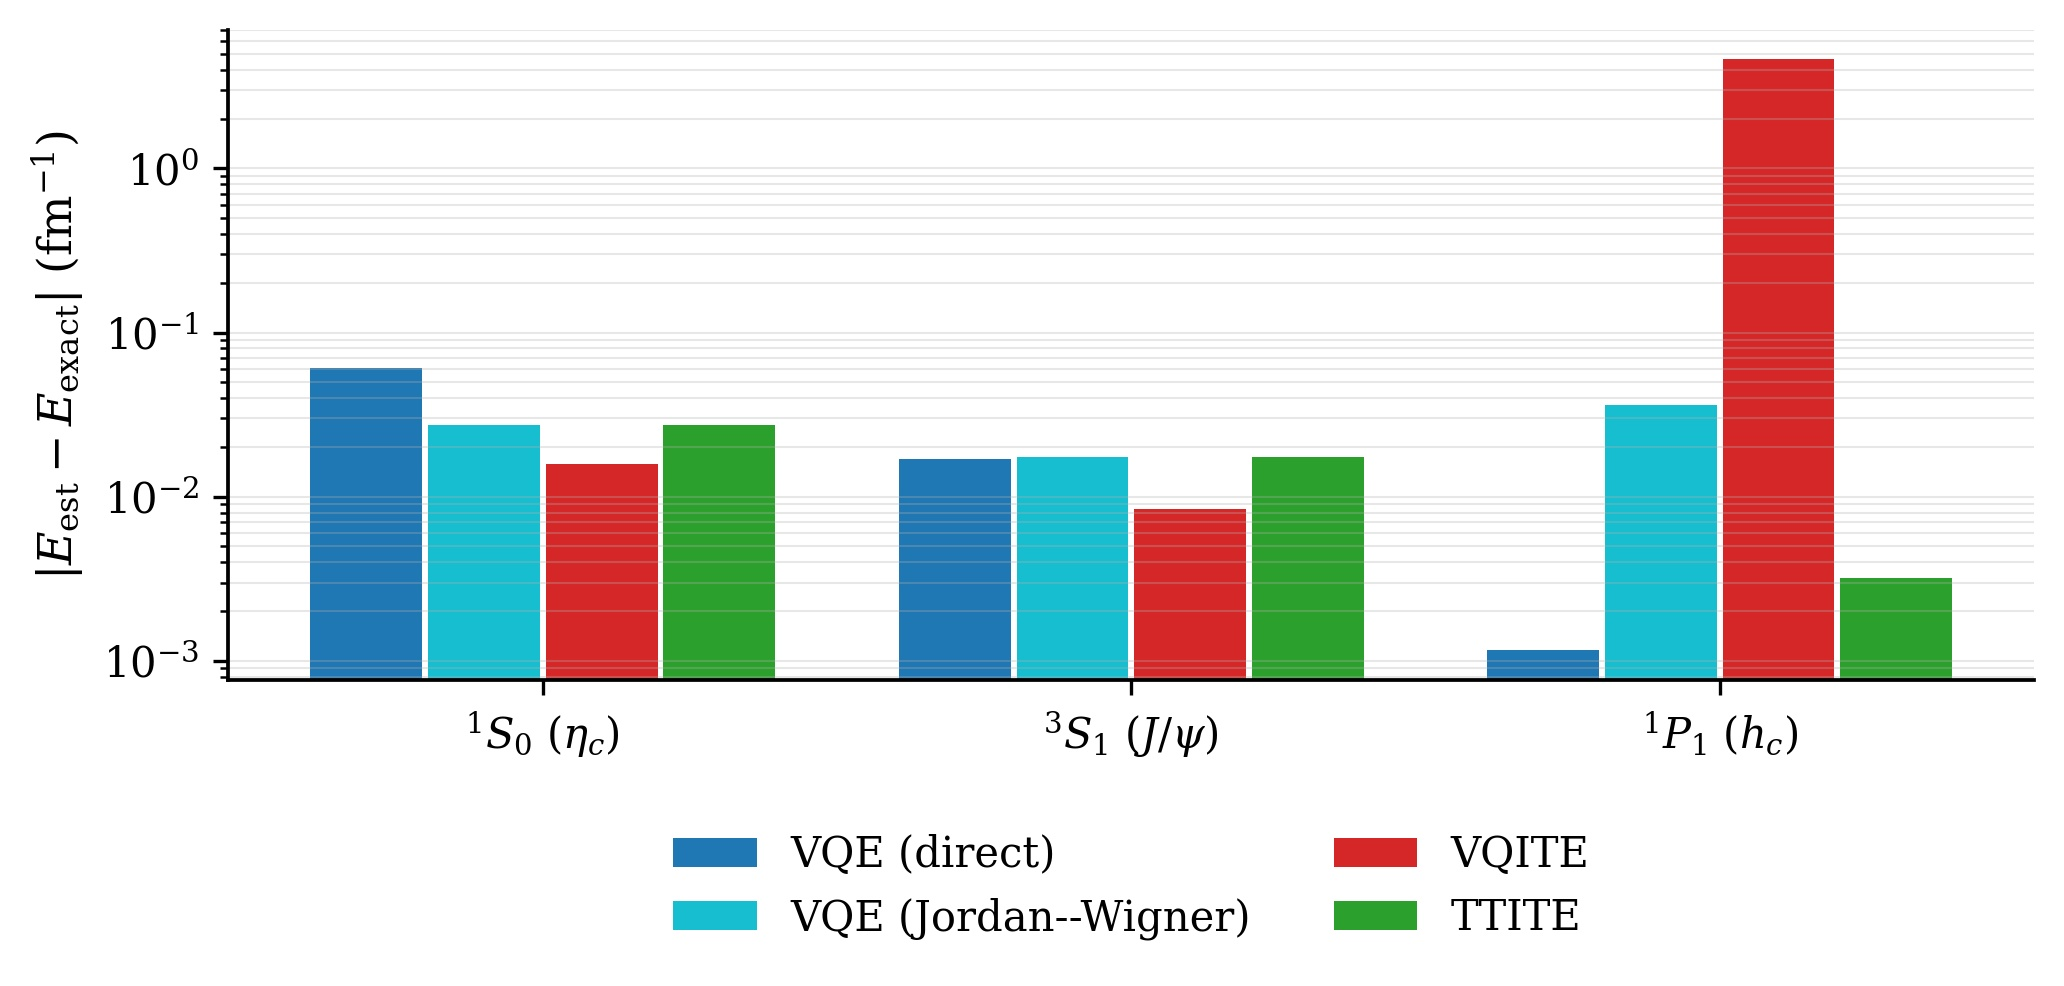
\includegraphics[width=0.85\textwidth]{figures/energy_summary.jpeg}
\caption{Absolute ground-state energy error per (channel, method) in the
  noiseless simulator (log scale). TTITE saturates the simulation
  precision; the variational methods are bounded above by their ansatz
  expressibility.}
\label{fig:energy_summary}
\end{figure}

\subsection{Excited states}
\label{ssec:excited}

We compute the four lowest eigenvalues per channel using the
orthogonalisation/penalty strategy of \cref{ssec:vqe_excited}. Both
VQE encodings are run; the VQITE column of \cref{tab:excited} is
reserved for follow-up work---the same penalty machinery
(\cref{eq:penalised_H}) applies, but the per-step circuit overhead
makes a full sweep impractical within the time budget of this thesis.
TTITE does not support excited states directly and is omitted from
this table.

\begin{table}[htbp]
\centering
\caption{Ground and excited-state energies (fm$^{-1}$) obtained by
  penalty-based VQE. $E_{\mathrm{exact}}$ is the eigenvalue of the
  classical $4\times 4$ diagonalisation. ``--'' entries are reserved
  for VQITE, which is left for future work.}
\label{tab:excited}
\renewcommand{\arraystretch}{1.15}
\small
\begin{tabular}{llrrrr}
\toprule
Channel & $k$ & $E_{\mathrm{exact}}$ & VQE     & VQE-JW  & VQITE \\
\midrule
\multirow{4}{*}{${}^1S_0$}
& $0$ & $0.391$ & $0.429$ & $0.472$ & --- \\
& $1$ & $3.483$ & $3.489$ & $3.466$ & --- \\
& $2$ & $5.643$ & $5.573$ & $5.519$ & --- \\
& $3$ & $7.545$ & $7.048$ & $7.509$ & --- \\
\midrule
\multirow{4}{*}{${}^3S_1$}
& $0$ & $0.752$ & $0.808$ & $0.776$ & --- \\
& $1$ & $3.633$ & $3.656$ & $3.678$ & --- \\
& $2$ & $5.727$ & $7.458$ & $5.927$ & --- \\
& $3$ & $7.646$ & $5.660$ & $6.179$ & --- \\
\midrule
\multirow{4}{*}{${}^1P_1$}
& $0$ & $2.781$ & $2.798$ & $2.772$ & --- \\
& $1$ & $4.883$ & $4.889$ & $4.923$ & --- \\
& $2$ & $6.756$ & $7.882$ & $6.779$ & --- \\
& $3$ & $8.770$ & $7.058$ & $5.613$ & --- \\
\bottomrule
\end{tabular}
\end{table}

\begin{figure}[htbp]
\centering
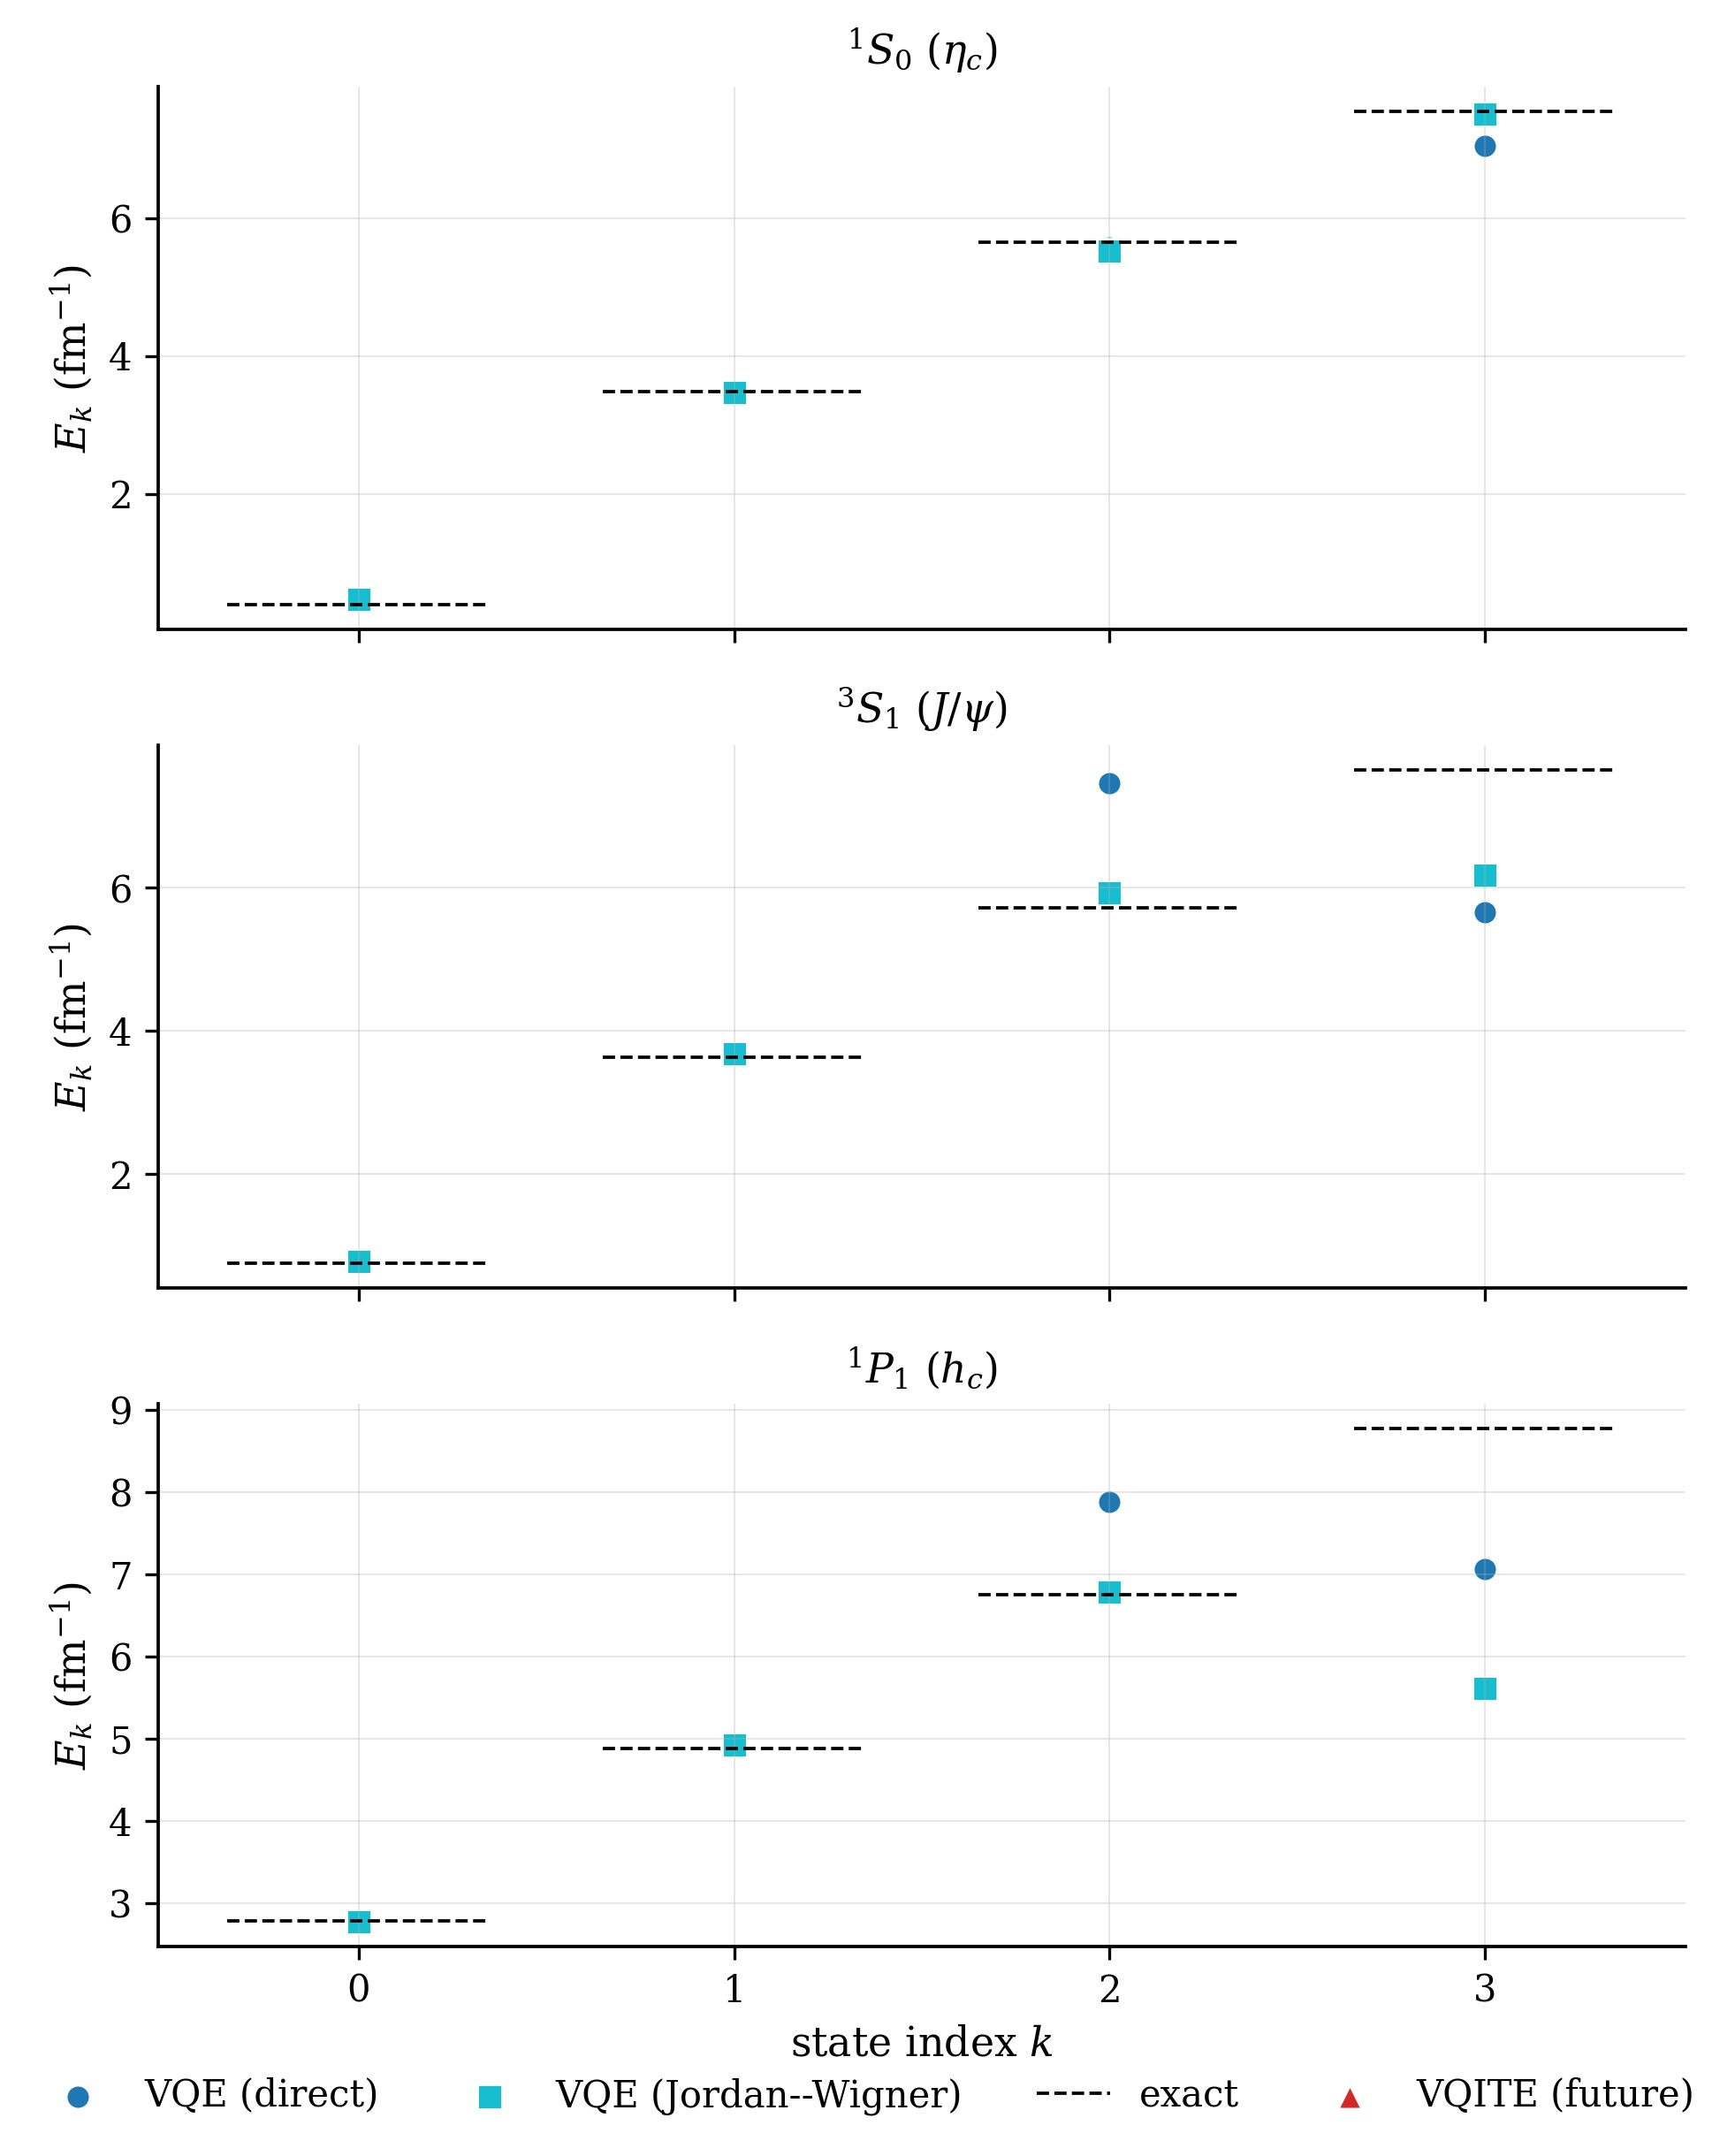
\includegraphics[width=\textwidth]{figures/excited_states.jpeg}
\caption{Energy-level diagram for the three channels. Black dashes mark
  the exact eigenvalues; coloured markers are the penalty-based VQE
  estimates in both encodings. The slot for VQITE excited states is
  preserved for follow-up work.}
\label{fig:excited}
\end{figure}

\Cref{fig:excited} shows the same information graphically. The ground
and first excited states are recovered with errors of at most
$\sim 0.08$~fm$^{-1}$ across all channels and both encodings. Higher
states ($k=2,3$) are more difficult: the penalty cost in
\cref{eq:penalised_H} stiffens the optimisation landscape as the
already-found subspace grows, and gradient-free COBYLA can converge to
the wrong eigenstate of the constrained problem. In several
${}^3S_1$ and ${}^1P_1$ entries the penalty method exchanges the
identities of $k=2$ and $k=3$ (e.g.\ VQE on ${}^3S_1$ assigns
$E_2 \approx 7.5$, near the exact $E_3 = 7.65$, and $E_3 \approx 5.7$,
near the exact $E_2 = 5.73$). VQE-JW is noticeably more reliable on
the third level for ${}^1S_0$ and ${}^1P_1$, though it inherits the
same $k=3$ degradation elsewhere.

% ──────────────────────────────────────────────────────────────────
\section{Noisy benchmark}
\label{sec:noisy}

We now switch the simulator backend to
\texttt{AerSimulator(noise\_model=make\_noise\_model($p$))} and re-run
the ground-state computation for each method at the five depolarising
rates listed in \cref{sec:results-setup}. \Cref{fig:noise-energy}
plots the absolute energy error against $p$ for the three channels;
\cref{fig:noise-fidelity} plots the fidelity. The Jordan--Wigner VQE
variant is omitted from the sweep, since its circuit class is similar
to the direct-encoding VQE and the qualitative noise response is the
same; the per-method noise behaviour discussed below applies to it as
well.

\begin{figure}[htbp]
\centering
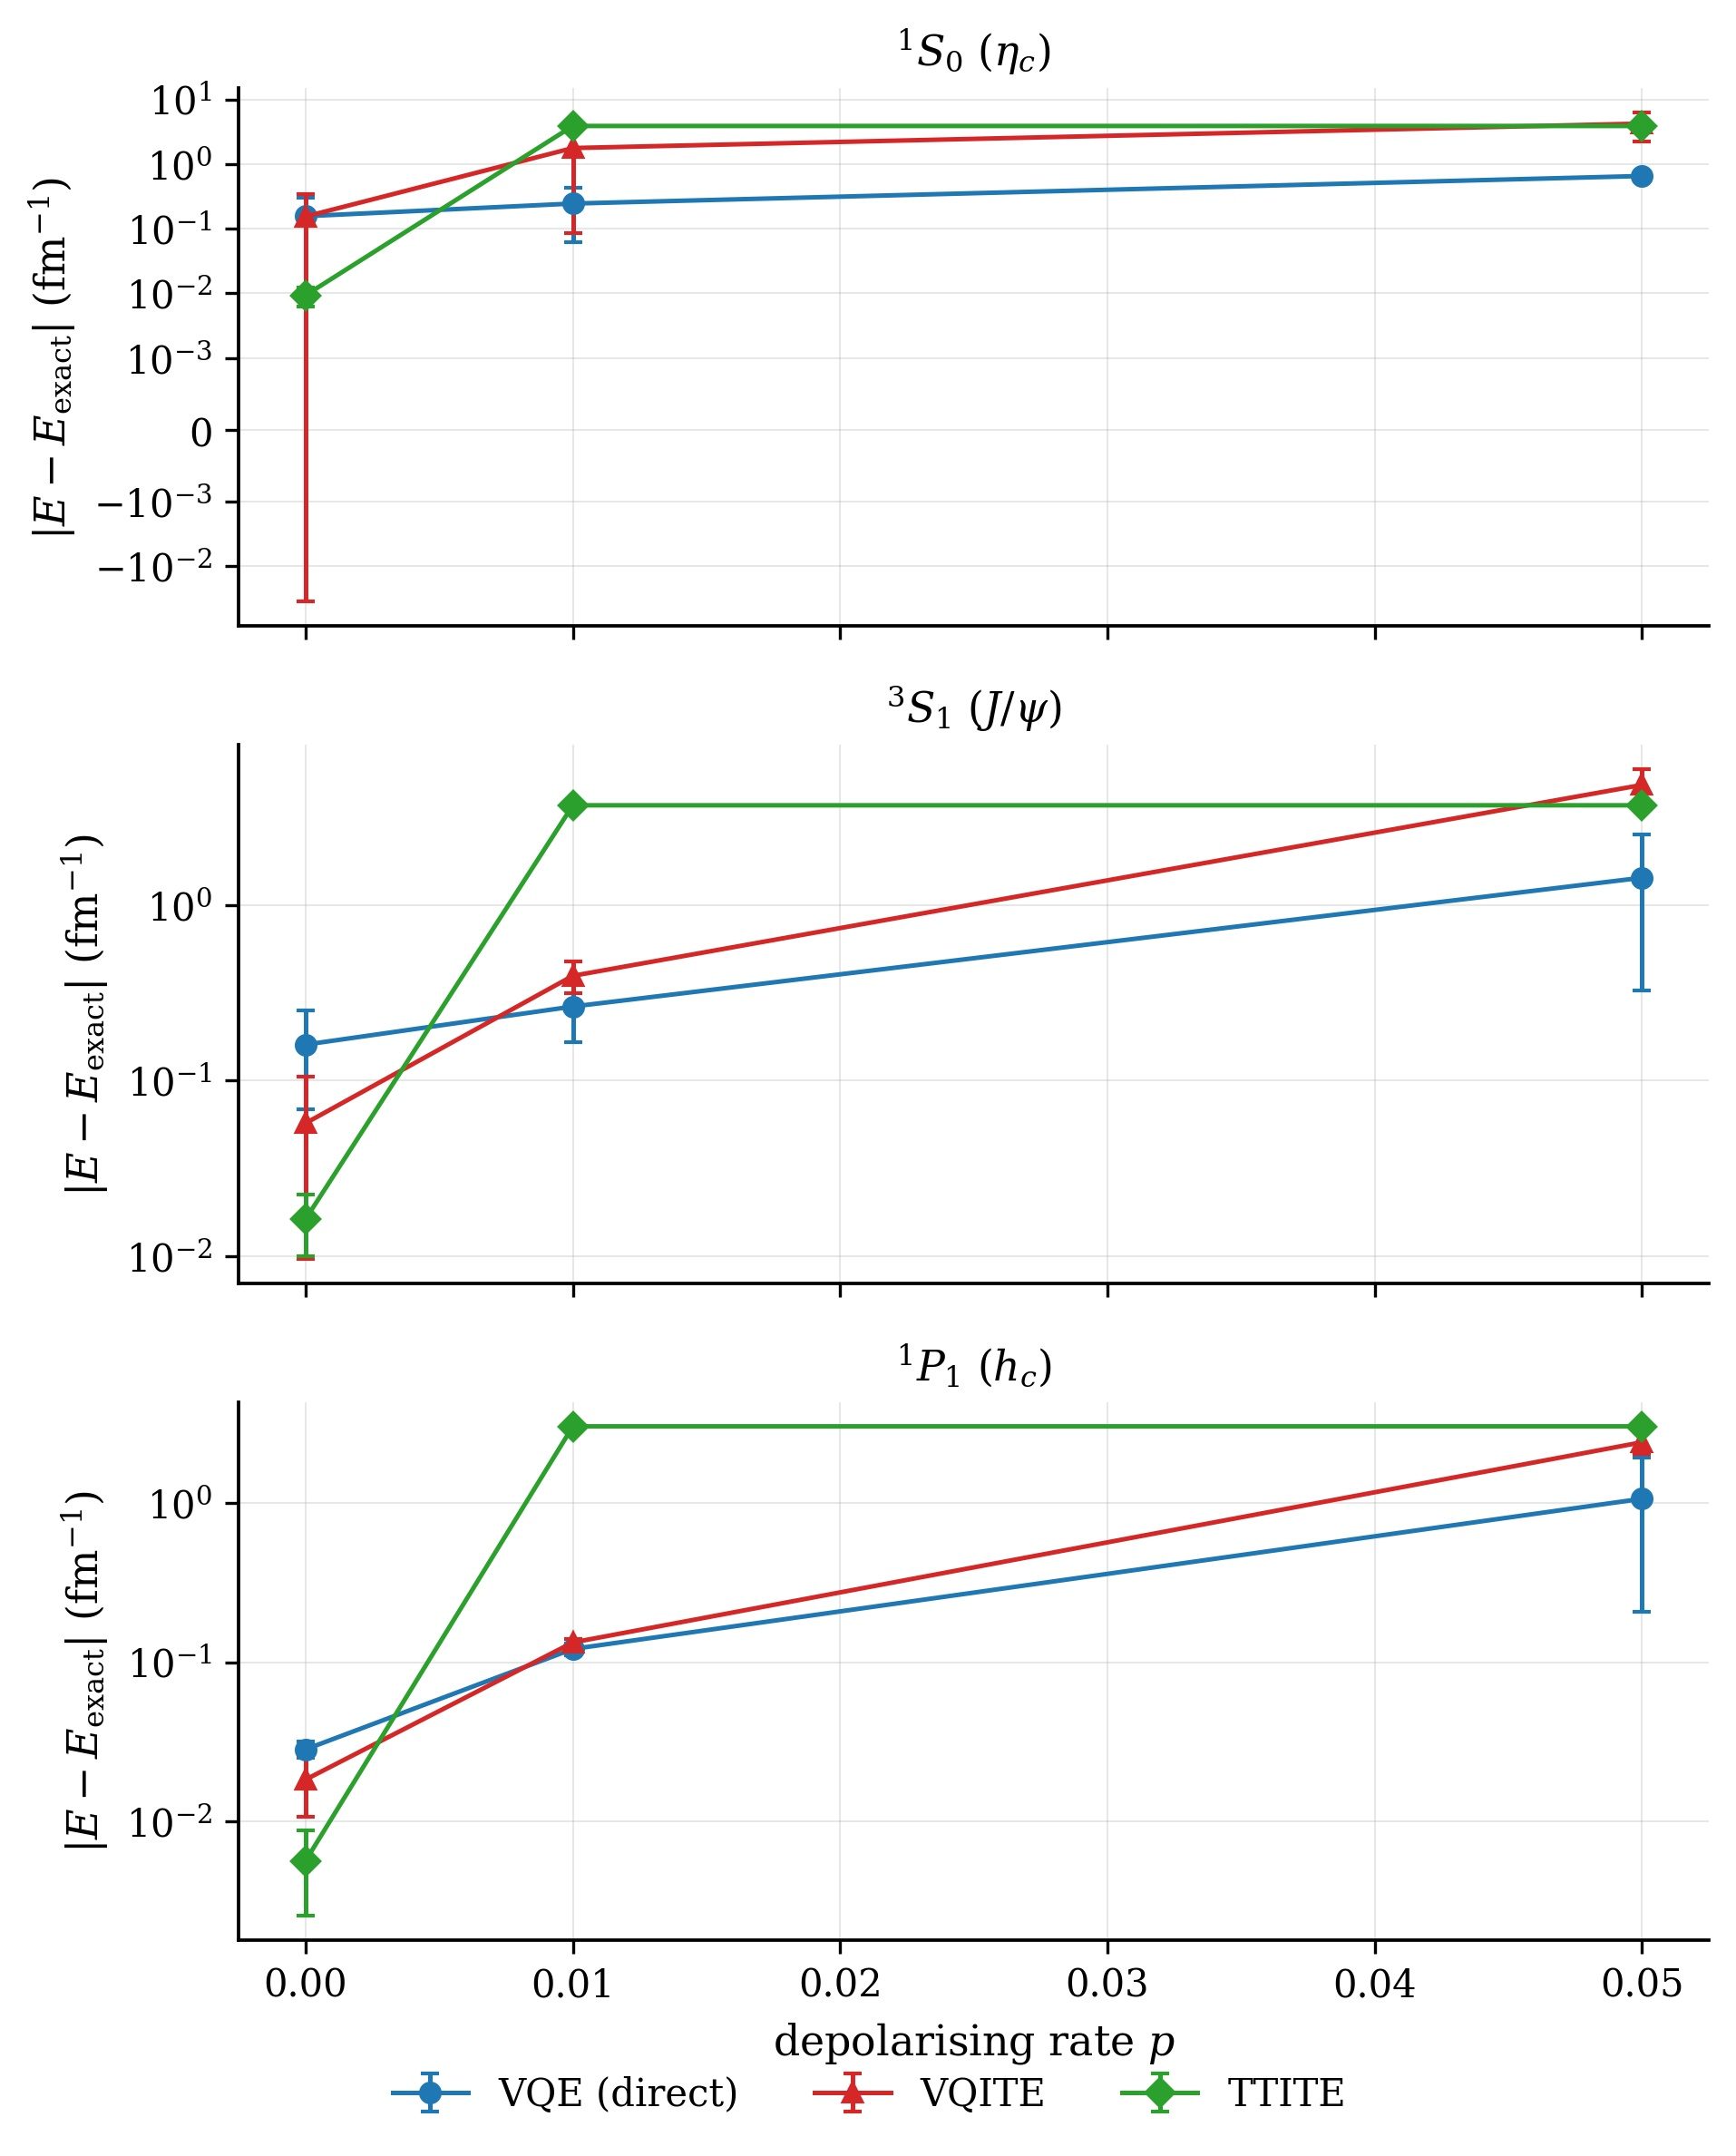
\includegraphics[width=\textwidth]{figures/noise_sweep_energy.jpeg}
\caption{Absolute energy error vs.\ depolarising rate $p$ for each
  channel. Error bars are the standard deviation over three repeats.
  The $y$-axis is symmetric-log to capture both the sub-$10^{-3}$
  noiseless regime and the $\mathcal{O}(1)$ degradation at $p = 0.05$.}
\label{fig:noise-energy}
\end{figure}

\begin{figure}[htbp]
\centering
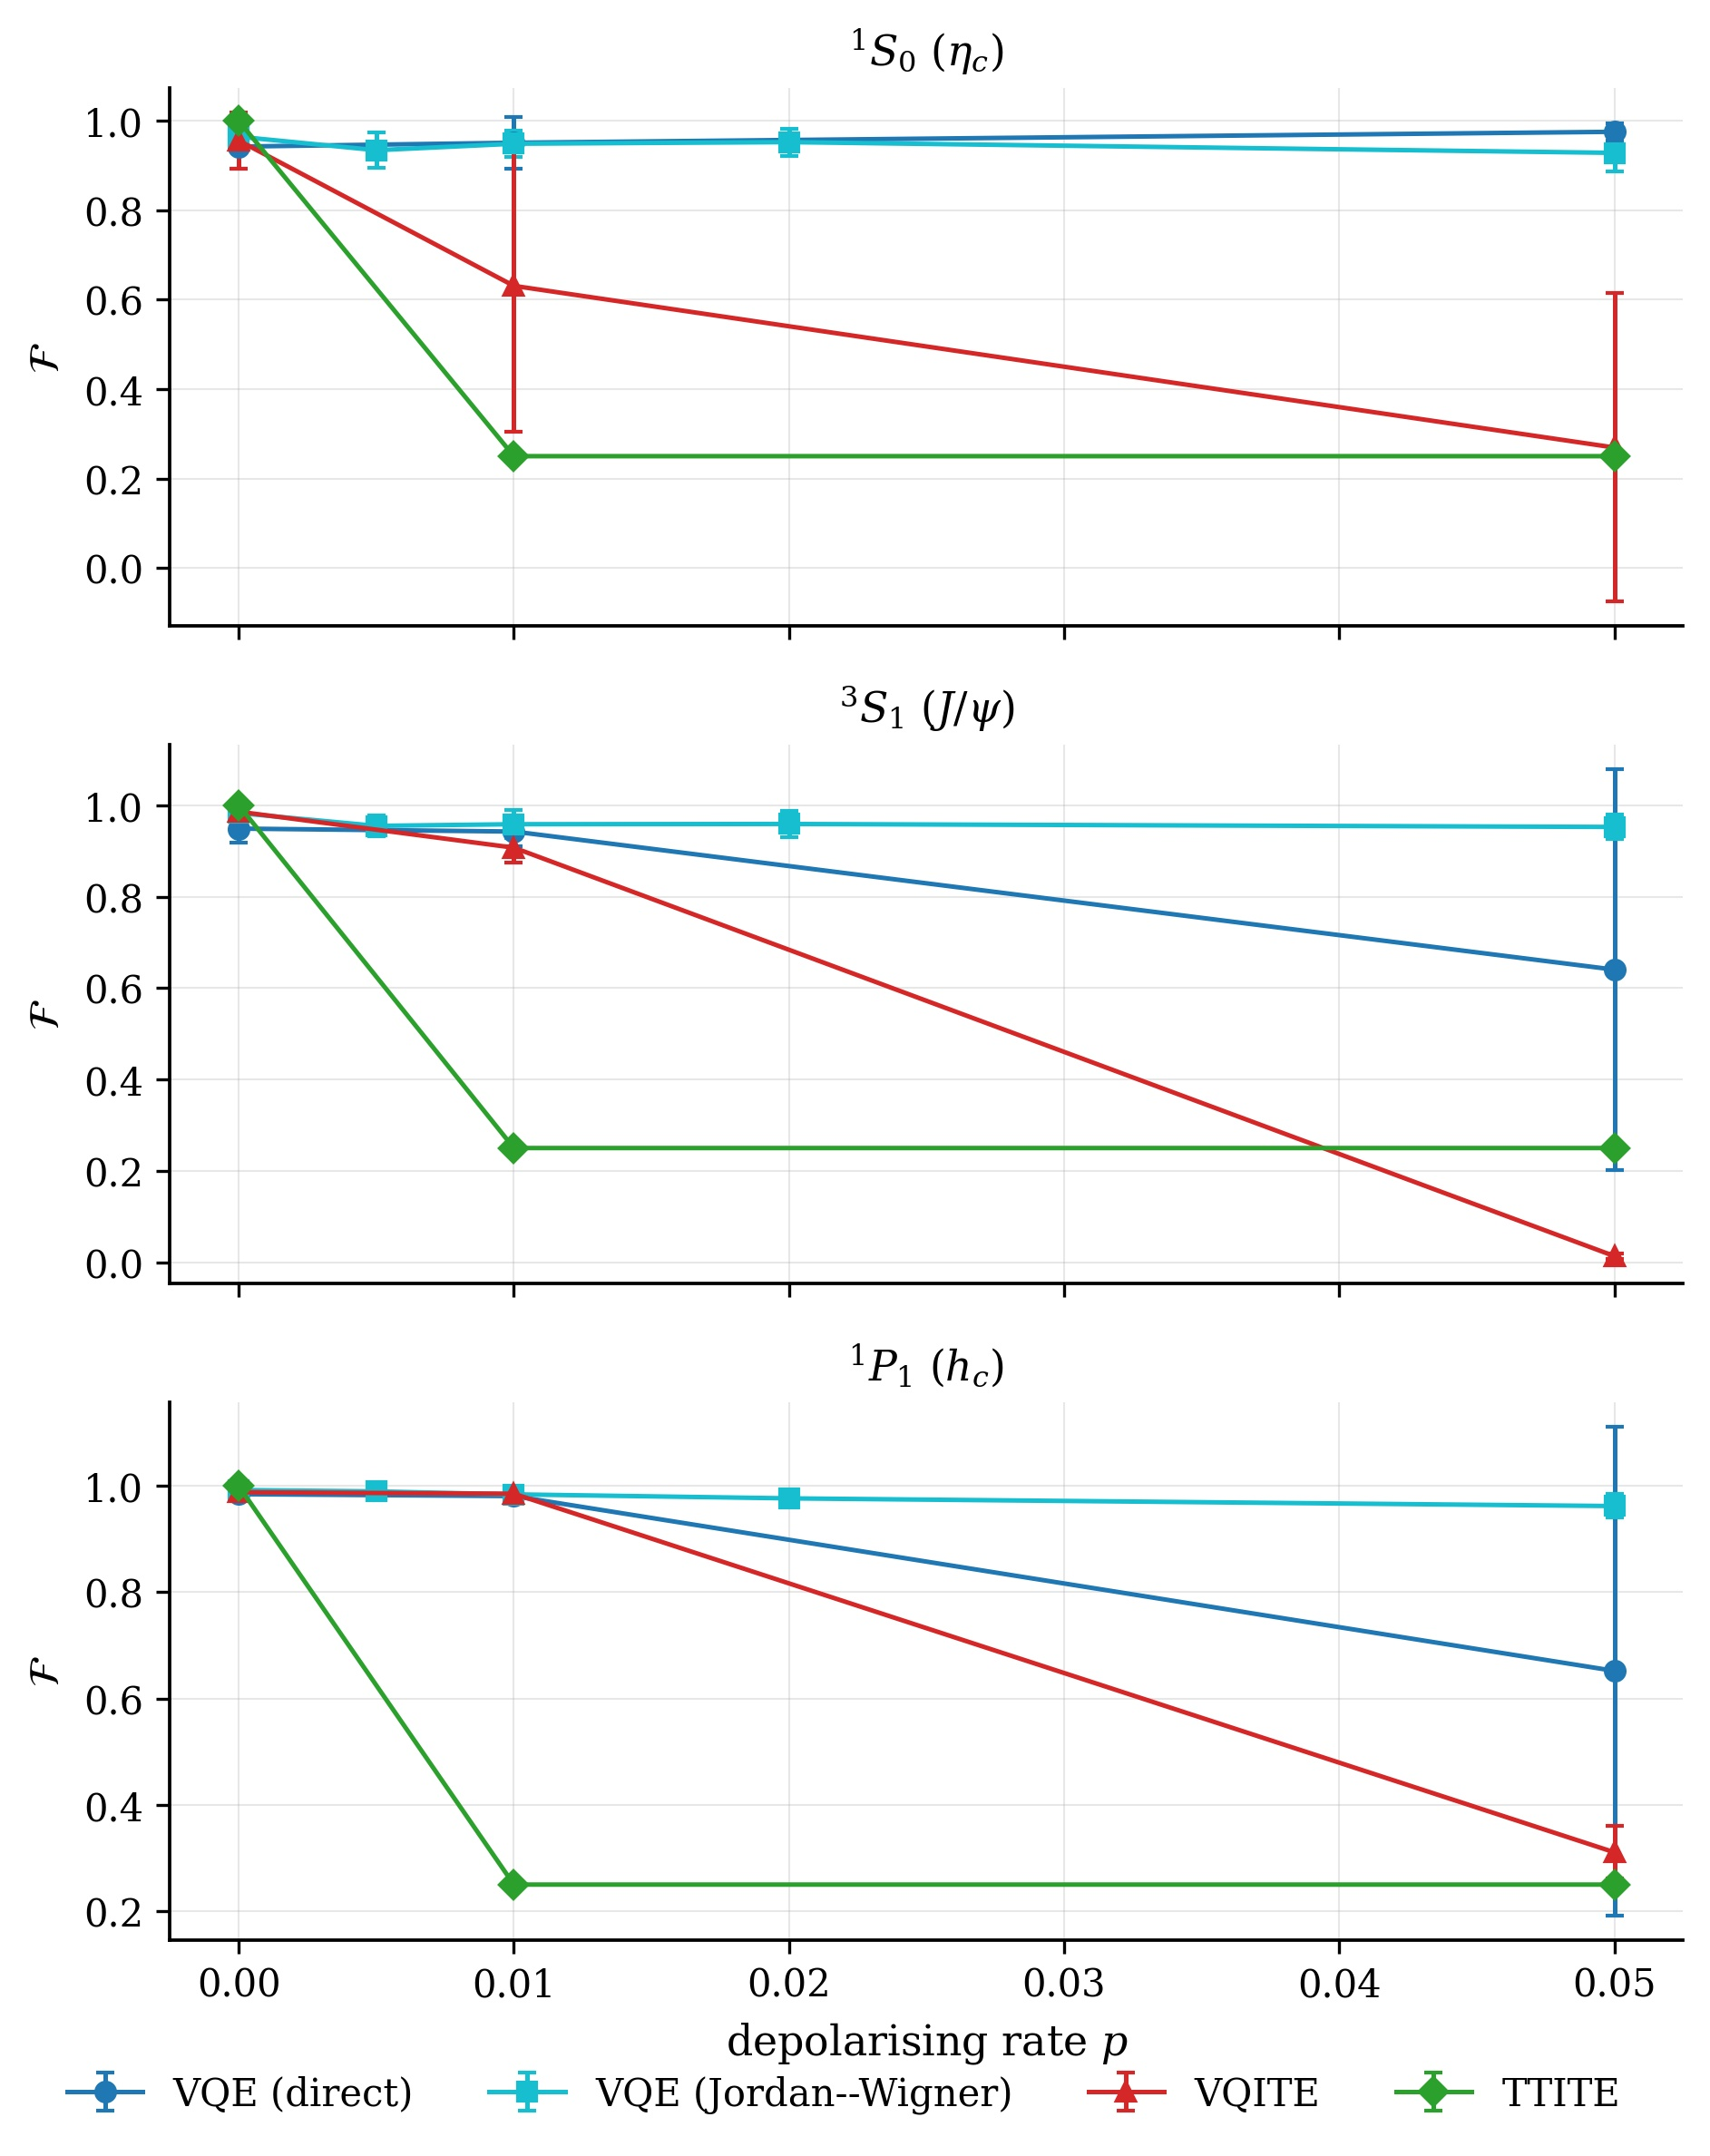
\includegraphics[width=\textwidth]{figures/noise_sweep_fidelity.jpeg}
\caption{Ground-state fidelity vs.\ depolarising rate $p$ for each
  channel. Error bars are the standard deviation over three repeats.}
\label{fig:noise-fidelity}
\end{figure}

The three algorithms degrade in qualitatively different ways. VQE is
the most resilient: its shallow ansatz (\cref{fig:woloshyn_ansatz}) is
exposed to only $\mathcal{O}(1)$ gates per energy evaluation, and the
gradient-free optimiser absorbs the resulting shot+gate noise into the
search. VQITE degrades faster because the metric tensor and
parameter-shift estimates of \cref{eq:metric_fd,eq:param_shift} both
require differences of noisy expectation values, so its effective
signal-to-noise ratio drops more sharply with $p$. TTITE collapses
catastrophically: with $\sim\!2{,}250$ sequential noisy gates over a
full Trotter trajectory and post-selection that cannot reject failed
LCU branches on real hardware, the work register relaxes toward the
maximally mixed state $\mathrm{Tr}(H)/4$, and the fidelity drops to
${\sim}\,0.25$ (random guessing in the 4-d Hilbert space) at any
non-zero noise rate.

% ──────────────────────────────────────────────────────────────────
\section{Summary}
\label{sec:results-summary}

In the noiseless regime all four methods reproduce the channel
eigenvalues, but they are not interchangeable: TTITE is essentially
exact (limited by simulation precision), VQE in either encoding is
limited by the chosen ansatz at the $\sim 10^{-2}$~fm$^{-1}$ level,
and VQITE accuracy is channel dependent because the metric tensor is
sensitive to the shape of the energy landscape. Under depolarising
noise the ranking inverts: VQE is the most resilient and TTITE the
most fragile, with the cross-over already at $p \lesssim 10^{-2}$.
These observations motivate the noise-mitigation strategies developed
in the next chapter.
   % Results
% \input{chapter4}   % Noise and Error Mitigation
% \input{chapter5}   % Conclusions and Outlook

% ── Bibliography ──
\printbibliography[heading=bibintoc]

\end{document}
